%%%%%%%%%%%%%%%%%%%%%%%%%%%%%%%%%%%%%%%%%
% The Legrand Orange Book
% LaTeX Template
% Version 2.1.1 (14/2/16)
%
% This template has been downloaded from:
% http://www.LaTeXTemplates.com
%
% Original author:
% Mathias Legrand (legrand.mathias@gmail.com) with modifications by:
% Vel (vel@latextemplates.com)
%
% License:
% CC BY-NC-SA 3.0 (http://creativecommons.org/licenses/by-nc-sa/3.0/)
%
% Compiling this template:
% This template uses biber for its bibliography and makeindex for its index.
% When you first open the template, compile it from the command line with the 
% commands below to make sure your LaTeX distribution is configured correctly:
%
% 1) pdflatex main
% 2) makeindex main.idx -s StyleInd.ist
% 3) biber main
% 4) pdflatex main x 2
%
% After this, when you wish to update the bibliography/index use the appropriate
% command above and make sure to compile with pdflatex several times 
% afterwards to propagate your changes to the document.
%
% This template also uses a number of packages which may need to be
% updated to the newest versions for the template to compile. It is strongly
% recommended you update your LaTeX distribution if you have any
% compilation errors.
%
% Important note:
% Chapter heading images should have a 2:1 width:height ratio,
% e.g. 920px width and 460px height.
%
%%%%%%%%%%%%%%%%%%%%%%%%%%%%%%%%%%%%%%%%%

%----------------------------------------------------------------------------------------
%	PACKAGES AND OTHER DOCUMENT CONFIGURATIONS
%----------------------------------------------------------------------------------------

\documentclass[11pt,fleqn]{book} % Default font size and left-justified equations

\newcommand{\mainagent}{simulation agent}
\newcommand{\MainAgent}{Simulation Agent}
\newcommand{\TimeAgent}{Time Agent}
\newcommand{\TimeSteppingAgent}{TimeSteppingAgent}
\newcommand{\SimpleCommunicationAgent}{SimpleCommunicationAgent}
\newcommand{\CommunicationAgent}{Communication Agent}
\newcommand{\InterdependentCommunicationAgent}{InterdependentCommunicationAgent}
\newcommand{\TokenCommunicationAgent}{TokenCommunicationAgent}
\newcommand{\DomainAgent}{Domain Agent} % e.g. InterpssFlowDomainAgent
\newcommand{\NegotiatorAgent}{Negotiator Agent}
\newcommand{\InterpssDomainAgent}{InterpssBackend}
\newcommand{\MatpowerDomainAgent}{MatpowerBackend}
\newcommand{\BenchmarkAgent}{BenchmarkSimulationAgent}
\newcommand{\BenchmarkLogReplayer}{BenchmarkLogReplayer}
\newcommand{\CascadeAgent}{CascadeAgent}
\newcommand{\Backend}[1][]{Backend#1} % general name for backend, variable for plural
\newcommand{\backend}[1][]{backend#1}
\newcommand{\Domain}[1][]{Domain#1} % general name for domain
\newcommand{\domain}[1][]{domain#1}
\newcommand{\backendparameters}{domain parameters}
\newcommand{\BackendParameterLoader}{BackendParameterLoader}
\newcommand{\backendParametersFile}{backendParameters.txt}
%----------------------------------------------------------------------------------------

%%%%%%%%%%%%%%%%%%%%%%%%%%%%%%%%%%%%%%%%%
% The Legrand Orange Book
% Structural Definitions File
% Version 2.0 (9/2/15)
%
% Original author:
% Mathias Legrand (legrand.mathias@gmail.com) with modifications by:
% Vel (vel@latextemplates.com)
% 
% This file has been downloaded from:
% http://www.LaTeXTemplates.com
%
% License:
% CC BY-NC-SA 3.0 (http://creativecommons.org/licenses/by-nc-sa/3.0/)
%
%%%%%%%%%%%%%%%%%%%%%%%%%%%%%%%%%%%%%%%%%

%----------------------------------------------------------------------------------------
%	VARIOUS REQUIRED PACKAGES AND CONFIGURATIONS
%----------------------------------------------------------------------------------------
\usepackage{multirow}

\usepackage[top=3cm,bottom=3cm,left=3cm,right=3cm,headsep=10pt,a4paper]{geometry} % Page margins

\usepackage{graphicx} % Required for including pictures
\graphicspath{{Pictures/}} % Specifies the directory where pictures are stored

\usepackage{lipsum} % Inserts dummy text

\usepackage{tikz} % Required for drawing custom shapes

\usepackage[english]{babel} % English language/hyphenation

\usepackage{enumitem} % Customize lists
\setlist{nolistsep} % Reduce spacing between bullet points and numbered lists

\usepackage{booktabs} % Required for nicer horizontal rules in tables

\usepackage{xcolor, colortbl} % Required for specifying colors by name
\definecolor{ocre}{RGB}{243,102,25} % Define the orange color used for highlighting throughout the book
\definecolor{Gray}{gray}{0.85}
\usepackage{listings} % for displaying code blocks
\lstset{language=Java}
\lstset{basicstyle=\small}

\setlength{\parindent}{0cm}

\usepackage{tabto} %% utilize tabs (added by mark)

%----------------------------------------------------------------------------------------
%	FONTS
%----------------------------------------------------------------------------------------

\usepackage{avant} % Use the Avantgarde font for headings
%\usepackage{times} % Use the Times font for headings
\usepackage{mathptmx} % Use the Adobe Times Roman as the default text font together with math symbols from the Sym­bol, Chancery and Com­puter Modern fonts

\usepackage{microtype} % Slightly tweak font spacing for aesthetics
\usepackage[utf8]{inputenc} % Required for including letters with accents
\usepackage[T1]{fontenc} % Use 8-bit encoding that has 256 glyphs

%----------------------------------------------------------------------------------------
%	BIBLIOGRAPHY AND INDEX
%----------------------------------------------------------------------------------------

\usepackage[style=alphabetic,citestyle=numeric,sorting=nyt,sortcites=true,autopunct=true,babel=hyphen,hyperref=true,abbreviate=false,backref=true,backend=biber]{biblatex}
\addbibresource{bibliography.bib} % BibTeX bibliography file
\defbibheading{bibempty}{}

\usepackage{calc} % For simpler calculation - used for spacing the index letter headings correctly
\usepackage{makeidx} % Required to make an index
\makeindex % Tells LaTeX to create the files required for indexing

%----------------------------------------------------------------------------------------
%	MAIN TABLE OF CONTENTS
%----------------------------------------------------------------------------------------

\usepackage{titletoc} % Required for manipulating the table of contents

\contentsmargin{0cm} % Removes the default margin

% Part text styling
\titlecontents{part}[0cm]
{\addvspace{20pt}\centering\large\bfseries}
{}
{}
{}

% Chapter text styling
\titlecontents{chapter}[1.25cm] % Indentation
{\addvspace{12pt}\large\sffamily\bfseries} % Spacing and font options for chapters
{\color{ocre!60}\contentslabel[\Large\thecontentslabel]{1.25cm}\color{ocre}} % Chapter number
{\color{ocre}}  
{\color{ocre!60}\normalsize\;\titlerule*[.5pc]{.}\;\thecontentspage} % Page number

% Section text styling
\titlecontents{section}[1.25cm] % Indentation
{\addvspace{3pt}\sffamily\bfseries} % Spacing and font options for sections
{\contentslabel[\thecontentslabel]{1.25cm}} % Section number
{}
{\hfill\color{black}\thecontentspage} % Page number
[]

% Subsection text styling
\titlecontents{subsection}[1.25cm] % Indentation
{\addvspace{1pt}\sffamily\small} % Spacing and font options for subsections
{\contentslabel[\thecontentslabel]{1.25cm}} % Subsection number
{}
{\ \titlerule*[.5pc]{.}\;\thecontentspage} % Page number
[]

% List of figures
\titlecontents{figure}[0em]
{\addvspace{-5pt}\sffamily}
{\thecontentslabel\hspace*{1em}}
{}
{\ \titlerule*[.5pc]{.}\;\thecontentspage}
[]

% List of tables
\titlecontents{table}[0em]
{\addvspace{-5pt}\sffamily}
{\thecontentslabel\hspace*{1em}}
{}
{\ \titlerule*[.5pc]{.}\;\thecontentspage}
[]

%----------------------------------------------------------------------------------------
%	MINI TABLE OF CONTENTS IN PART HEADS
%----------------------------------------------------------------------------------------

% Chapter text styling
\titlecontents{lchapter}[0em] % Indenting
{\addvspace{15pt}\large\sffamily\bfseries} % Spacing and font options for chapters
{\color{ocre}\contentslabel[\Large\thecontentslabel]{1.25cm}\color{ocre}} % Chapter number
{}  
{\color{ocre}\normalsize\sffamily\bfseries\;\titlerule*[.5pc]{.}\;\thecontentspage} % Page number

% Section text styling
\titlecontents{lsection}[0em] % Indenting
{\sffamily\small} % Spacing and font options for sections
{\contentslabel[\thecontentslabel]{1.25cm}} % Section number
{}
{}

% Subsection text styling
\titlecontents{lsubsection}[.5em] % Indentation
{\normalfont\footnotesize\sffamily} % Font settings
{}
{}
{}

%----------------------------------------------------------------------------------------
%	PAGE HEADERS
%----------------------------------------------------------------------------------------

\usepackage{fancyhdr} % Required for header and footer configuration

\pagestyle{fancy}
\renewcommand{\chaptermark}[1]{\markboth{\sffamily\normalsize\bfseries\chaptername\ \thechapter.\ #1}{}} % Chapter text font settings
\renewcommand{\sectionmark}[1]{\markright{\sffamily\normalsize\thesection\hspace{5pt}#1}{}} % Section text font settings
\fancyhf{} \fancyhead[LE,RO]{\sffamily\normalsize\thepage} % Font setting for the page number in the header
\fancyhead[LO]{\rightmark} % Print the nearest section name on the left side of odd pages
\fancyhead[RE]{\leftmark} % Print the current chapter name on the right side of even pages
\renewcommand{\headrulewidth}{0.5pt} % Width of the rule under the header
\addtolength{\headheight}{2.5pt} % Increase the spacing around the header slightly
\renewcommand{\footrulewidth}{0pt} % Removes the rule in the footer
\fancypagestyle{plain}{\fancyhead{}\renewcommand{\headrulewidth}{0pt}} % Style for when a plain pagestyle is specified

% Removes the header from odd empty pages at the end of chapters
\makeatletter
\renewcommand{\cleardoublepage}{
\clearpage\ifodd\c@page\else
\hbox{}
\vspace*{\fill}
\thispagestyle{empty}
%\newpage
\fi}

%----------------------------------------------------------------------------------------
%	THEOREM STYLES
%----------------------------------------------------------------------------------------

\usepackage{amsmath,amsfonts,amssymb,amsthm} % For math equations, theorems, symbols, etc

\newcommand{\intoo}[2]{\mathopen{]}#1\,;#2\mathclose{[}}
\newcommand{\ud}{\mathop{\mathrm{{}d}}\mathopen{}}
\newcommand{\intff}[2]{\mathopen{[}#1\,;#2\mathclose{]}}
\newtheorem{notation}{Notation}[chapter]

% Boxed/framed environments
\newtheoremstyle{ocrenumbox}% % Theorem style name
{0pt}% Space above
{0pt}% Space below
{\normalfont}% % Body font
{}% Indent amount
{\small\bf\sffamily\color{ocre}}% % Theorem head font
{\;}% Punctuation after theorem head
{0.25em}% Space after theorem head
{\small\sffamily\color{ocre}\thmname{#1}\nobreakspace\thmnumber{\@ifnotempty{#1}{}\@upn{#2}}% Theorem text (e.g. Theorem 2.1)
\thmnote{\nobreakspace\the\thm@notefont\sffamily\bfseries\color{black}---\nobreakspace#3.}} % Optional theorem note
\renewcommand{\qedsymbol}{$\blacksquare$}% Optional qed square

\newtheoremstyle{blacknumex}% Theorem style name
{5pt}% Space above
{5pt}% Space below
{\normalfont}% Body font
{} % Indent amount
{\small\bf\sffamily}% Theorem head font
{\;}% Punctuation after theorem head
{0.25em}% Space after theorem head
{\small\sffamily{\tiny\ensuremath{\blacksquare}}\nobreakspace\thmname{#1}\nobreakspace\thmnumber{\@ifnotempty{#1}{}\@upn{#2}}% Theorem text (e.g. Theorem 2.1)
\thmnote{\nobreakspace\the\thm@notefont\sffamily\bfseries---\nobreakspace#3.}}% Optional theorem note

\newtheoremstyle{blacknumbox} % Theorem style name
{0pt}% Space above
{0pt}% Space below
{\normalfont}% Body font
{}% Indent amount
{\small\bf\sffamily}% Theorem head font
{\;}% Punctuation after theorem head
{0.25em}% Space after theorem head
{\small\sffamily\thmname{#1}\nobreakspace\thmnumber{\@ifnotempty{#1}{}\@upn{#2}}% Theorem text (e.g. Theorem 2.1)
\thmnote{\nobreakspace\the\thm@notefont\sffamily\bfseries---\nobreakspace#3.}}% Optional theorem note

% Non-boxed/non-framed environments
\newtheoremstyle{ocrenum}% % Theorem style name
{5pt}% Space above
{5pt}% Space below
{\normalfont}% % Body font
{}% Indent amount
{\small\bf\sffamily\color{ocre}}% % Theorem head font
{\;}% Punctuation after theorem head
{0.25em}% Space after theorem head
{\small\sffamily\color{ocre}\thmname{#1}\nobreakspace\thmnumber{\@ifnotempty{#1}{}\@upn{#2}}% Theorem text (e.g. Theorem 2.1)
\thmnote{\nobreakspace\the\thm@notefont\sffamily\bfseries\color{black}---\nobreakspace#3.}} % Optional theorem note
\renewcommand{\qedsymbol}{$\blacksquare$}% Optional qed square
\makeatother

% Defines the theorem text style for each type of theorem to one of the three styles above
\newcounter{dummy} 
\numberwithin{dummy}{section}
\theoremstyle{ocrenumbox}
\newtheorem{theoremeT}[dummy]{Theorem}
\newtheorem{problem}{Problem}[chapter]
\newtheorem{exerciseT}{Exercise}[chapter]
\theoremstyle{blacknumex}
\newtheorem{exampleT}{Example}[chapter]
\theoremstyle{blacknumbox}
\newtheorem{vocabulary}{Vocabulary}[chapter]
\newtheorem{definitionT}{Definition}[section]
\newtheorem{corollaryT}[dummy]{Corollary}
\theoremstyle{ocrenum}
\newtheorem{proposition}[dummy]{Proposition}

%----------------------------------------------------------------------------------------
%	DEFINITION OF COLORED BOXES
%----------------------------------------------------------------------------------------

\RequirePackage[framemethod=default]{mdframed} % Required for creating the theorem, definition, exercise and corollary boxes

% Theorem box
\newmdenv[skipabove=7pt,
skipbelow=7pt,
backgroundcolor=black!5,
linecolor=ocre,
innerleftmargin=5pt,
innerrightmargin=5pt,
innertopmargin=5pt,
leftmargin=0cm,
rightmargin=0cm,
innerbottommargin=5pt]{tBox}

% Exercise box	  
\newmdenv[skipabove=7pt,
skipbelow=7pt,
rightline=false,
leftline=true,
topline=false,
bottomline=false,
backgroundcolor=ocre!10,
linecolor=ocre,
innerleftmargin=5pt,
innerrightmargin=5pt,
innertopmargin=5pt,
innerbottommargin=5pt,
leftmargin=0cm,
rightmargin=0cm,
linewidth=4pt]{eBox}	

% Definition box
\newmdenv[skipabove=7pt,
skipbelow=7pt,
rightline=false,
leftline=true,
topline=false,
bottomline=false,
linecolor=ocre,
innerleftmargin=5pt,
innerrightmargin=5pt,
innertopmargin=0pt,
leftmargin=0cm,
rightmargin=0cm,
linewidth=4pt,
innerbottommargin=0pt]{dBox}	

% Corollary box
\newmdenv[skipabove=7pt,
skipbelow=7pt,
rightline=false,
leftline=true,
topline=false,
bottomline=false,
linecolor=gray,
backgroundcolor=black!5,
innerleftmargin=5pt,
innerrightmargin=5pt,
innertopmargin=5pt,
leftmargin=0cm,
rightmargin=0cm,
linewidth=4pt,
innerbottommargin=5pt]{cBox}

% Creates an environment for each type of theorem and assigns it a theorem text style from the "Theorem Styles" section above and a colored box from above
\newenvironment{theorem}{\begin{tBox}\begin{theoremeT}}{\end{theoremeT}\end{tBox}}
\newenvironment{exercise}{\begin{eBox}\begin{exerciseT}}{\hfill{\color{ocre}\tiny\ensuremath{\blacksquare}}\end{exerciseT}\end{eBox}}				  
\newenvironment{definition}{\begin{dBox}\begin{definitionT}}{\end{definitionT}\end{dBox}}	
\newenvironment{example}{\begin{exampleT}}{\hfill{\tiny\ensuremath{\blacksquare}}\end{exampleT}}		
\newenvironment{corollary}{\begin{cBox}\begin{corollaryT}}{\end{corollaryT}\end{cBox}}	

%----------------------------------------------------------------------------------------
%	REMARK ENVIRONMENT
%----------------------------------------------------------------------------------------

\newenvironment{remark}{\par\vspace{10pt}\small % Vertical white space above the remark and smaller font size
\begin{list}{}{
\leftmargin=35pt % Indentation on the left
\rightmargin=25pt}\item\ignorespaces % Indentation on the right
\makebox[-2.5pt]{\begin{tikzpicture}[overlay]
\node[draw=ocre!60,line width=1pt,circle,fill=ocre!25,font=\sffamily\bfseries,inner sep=2pt,outer sep=0pt] at (-15pt,0pt){\textcolor{ocre}{R}};\end{tikzpicture}} % Orange R in a circle
\advance\baselineskip -1pt}{\end{list}\vskip5pt} % Tighter line spacing and white space after remark

%----------------------------------------------------------------------------------------
%	SECTION NUMBERING IN THE MARGIN
%----------------------------------------------------------------------------------------

\makeatletter
\renewcommand{\@seccntformat}[1]{\llap{\textcolor{ocre}{\csname the#1\endcsname}\hspace{1em}}}                    
\renewcommand{\section}{\@startsection{section}{1}{\z@}
{-4ex \@plus -1ex \@minus -.4ex}
{1ex \@plus.2ex }
{\normalfont\large\sffamily\bfseries}}
\renewcommand{\subsection}{\@startsection {subsection}{2}{\z@}
{-3ex \@plus -0.1ex \@minus -.4ex}
{0.5ex \@plus.2ex }
{\normalfont\sffamily\bfseries}}
\renewcommand{\subsubsection}{\@startsection {subsubsection}{3}{\z@}
{-2ex \@plus -0.1ex \@minus -.2ex}
{.2ex \@plus.2ex }
{\normalfont\small\sffamily\bfseries}}                        
\renewcommand\paragraph{\@startsection{paragraph}{4}{\z@}
{-2ex \@plus-.2ex \@minus .2ex}
{.1ex}
{\normalfont\small\sffamily\bfseries}}

%----------------------------------------------------------------------------------------
%	PART HEADINGS
%----------------------------------------------------------------------------------------

% numbered part in the table of contents
\newcommand{\@mypartnumtocformat}[2]{%
\setlength\fboxsep{0pt}%
\noindent\colorbox{ocre!20}{\strut\parbox[c][.7cm]{\ecart}{\color{ocre!70}\Large\sffamily\bfseries\centering#1}}\hskip\esp\colorbox{ocre!40}{\strut\parbox[c][.7cm]{\linewidth-\ecart-\esp}{\Large\sffamily\centering#2}}}%
%%%%%%%%%%%%%%%%%%%%%%%%%%%%%%%%%%
% unnumbered part in the table of contents
\newcommand{\@myparttocformat}[1]{%
\setlength\fboxsep{0pt}%
\noindent\colorbox{ocre!40}{\strut\parbox[c][.7cm]{\linewidth}{\Large\sffamily\centering#1}}}%
%%%%%%%%%%%%%%%%%%%%%%%%%%%%%%%%%%
\newlength\esp
\setlength\esp{4pt}
\newlength\ecart
\setlength\ecart{1.2cm-\esp}
\newcommand{\thepartimage}{}%
\newcommand{\partimage}[1]{\renewcommand{\thepartimage}{#1}}%
\def\@part[#1]#2{%
\ifnum \c@secnumdepth >-2\relax%
\refstepcounter{part}%
\addcontentsline{toc}{part}{\texorpdfstring{\protect\@mypartnumtocformat{\thepart}{#1}}{\partname~\thepart\ ---\ #1}}
\else%
\addcontentsline{toc}{part}{\texorpdfstring{\protect\@myparttocformat{#1}}{#1}}%
\fi%
\startcontents%
\markboth{}{}%
{\thispagestyle{empty}%
\begin{tikzpicture}[remember picture,overlay]%
\node at (current page.north west){\begin{tikzpicture}[remember picture,overlay]%	
\fill[ocre!20](0cm,0cm) rectangle (\paperwidth,-\paperheight);
\node[anchor=north] at (4cm,-3.25cm){\color{ocre!40}\fontsize{220}{100}\sffamily\bfseries\@Roman\c@part}; 
\node[anchor=south east] at (\paperwidth-1cm,-\paperheight+1cm){\parbox[t][][t]{8.5cm}{
\printcontents{l}{0}{\setcounter{tocdepth}{1}}%
}};
\node[anchor=north east] at (\paperwidth-1.5cm,-3.25cm){\parbox[t][][t]{15cm}{\strut\raggedleft\color{white}\fontsize{30}{30}\sffamily\bfseries#2}};
\end{tikzpicture}};
\end{tikzpicture}}%
\@endpart}
\def\@spart#1{%
\startcontents%
\phantomsection
{\thispagestyle{empty}%
\begin{tikzpicture}[remember picture,overlay]%
\node at (current page.north west){\begin{tikzpicture}[remember picture,overlay]%	
\fill[ocre!20](0cm,0cm) rectangle (\paperwidth,-\paperheight);
\node[anchor=north east] at (\paperwidth-1.5cm,-3.25cm){\parbox[t][][t]{15cm}{\strut\raggedleft\color{white}\fontsize{30}{30}\sffamily\bfseries#1}};
\end{tikzpicture}};
\end{tikzpicture}}
\addcontentsline{toc}{part}{\texorpdfstring{%
\setlength\fboxsep{0pt}%
\noindent\protect\colorbox{ocre!40}{\strut\protect\parbox[c][.7cm]{\linewidth}{\Large\sffamily\protect\centering #1\quad\mbox{}}}}{#1}}%
\@endpart}
\def\@endpart{} 
%Before  \@endpart{
%\vfil\newpage
%\if@twoside
%\if@openright
%\null
%\thispagestyle{empty}%
%\newpage
%\fi
%\fi
%\if@tempswa
%\twocolumn
%\fi}

%----------------------------------------------------------------------------------------
%	CHAPTER HEADINGS
%----------------------------------------------------------------------------------------

% A switch to conditionally include a picture, implemented by  Christian Hupfer
\newif\ifusechapterimage
\usechapterimagetrue
\newcommand{\thechapterimage}{}%
\newcommand{\chapterimage}[1]{\ifusechapterimage\renewcommand{\thechapterimage}{#1}\fi}%
\def\@makechapterhead#1{%
{\parindent \z@ \raggedright \normalfont
\ifnum \c@secnumdepth >\m@ne
\if@mainmatter
\begin{tikzpicture}[remember picture,overlay]
\node at (current page.north west)
{\begin{tikzpicture}[remember picture,overlay]
\node[anchor=north west,inner sep=0pt] at (0,0) {\ifusechapterimage\includegraphics[width=\paperwidth]{\thechapterimage}\fi};
\draw[anchor=west] (\Gm@lmargin,-9cm) node [line width=2pt,rounded corners=15pt,draw=ocre,fill=white,fill opacity=0.5,inner sep=15pt]{\strut\makebox[22cm]{}};
\draw[anchor=west] (\Gm@lmargin+.3cm,-9cm) node {\huge\sffamily\bfseries\color{black}\thechapter. #1\strut};
\end{tikzpicture}};
\end{tikzpicture}
\else
\begin{tikzpicture}[remember picture,overlay]
\node at (current page.north west)
{\begin{tikzpicture}[remember picture,overlay]
\node[anchor=north west,inner sep=0pt] at (0,0) {\ifusechapterimage\includegraphics[width=\paperwidth]{\thechapterimage}\fi};
\draw[anchor=west] (\Gm@lmargin,-9cm) node [line width=2pt,rounded corners=15pt,draw=ocre,fill=white,fill opacity=0.5,inner sep=15pt]{\strut\makebox[22cm]{}};
\draw[anchor=west] (\Gm@lmargin+.3cm,-9cm) node {\huge\sffamily\bfseries\color{black}#1\strut};
\end{tikzpicture}};
\end{tikzpicture}
\fi\fi\par\vspace*{270\p@}}}

%-------------------------------------------

\def\@makeschapterhead#1{%
\begin{tikzpicture}[remember picture,overlay]
\node at (current page.north west)
{\begin{tikzpicture}[remember picture,overlay]
\node[anchor=north west,inner sep=0pt] at (0,0) {\ifusechapterimage\includegraphics[width=\paperwidth]{\thechapterimage}\fi};
\draw[anchor=west] (\Gm@lmargin,-9cm) node [line width=2pt,rounded corners=15pt,draw=ocre,fill=white,fill opacity=0.5,inner sep=15pt]{\strut\makebox[22cm]{}};
\draw[anchor=west] (\Gm@lmargin+.3cm,-9cm) node {\huge\sffamily\bfseries\color{black}#1\strut};
\end{tikzpicture}};
\end{tikzpicture}
\par\vspace*{270\p@}}
\makeatother

%----------------------------------------------------------------------------------------
%	HYPERLINKS IN THE DOCUMENTS
%----------------------------------------------------------------------------------------

\usepackage{hyperref}
\hypersetup{hidelinks,backref=true,pagebackref=true,hyperindex=true,colorlinks=false,breaklinks=true,urlcolor= ocre,bookmarks=true,bookmarksopen=false,pdftitle={Title},pdfauthor={Author}}
\usepackage{bookmark}
\bookmarksetup{
open,
numbered,
addtohook={%
\ifnum\bookmarkget{level}=0 % chapter
\bookmarksetup{bold}%
\fi
\ifnum\bookmarkget{level}=-1 % part
\bookmarksetup{color=ocre,bold}%
\fi
}
}
 % Insert the commands.tex file which contains the majority of the structure behind the template

\begin{document}

%----------------------------------------------------------------------------------------
%	TITLE PAGE
%----------------------------------------------------------------------------------------

\begingroup
\thispagestyle{empty}
\begin{tikzpicture}[remember picture,overlay]
\coordinate [below=12cm] (midpoint) at (current page.north);
\node at (current page.north west)
{\begin{tikzpicture}[remember picture,overlay]
\node[anchor=north west,inner sep=0pt] at (0,0) {
\includegraphics[width=\paperwidth]{background}}; % Background image
\draw[anchor=north] (midpoint) node [fill=ocre!30!white,fill opacity=0.6,text opacity=1,inner sep=1cm]{\Huge\centering\bfseries\sffamily\parbox[c][][t]{\paperwidth}{\centering SFINA Manual\\[15pt] % Book title
{\Large Simulation Framework for Intelligent Network Adaptations}\\[20pt] % Subtitle
{\Large Chair of Computational Social Science, ETH Zurich }}}; % Author name
\end{tikzpicture}};
\end{tikzpicture}
\vfill
\endgroup
%
%%----------------------------------------------------------------------------------------
%%	COPYRIGHT PAGE
%%----------------------------------------------------------------------------------------
%
%\newpage
%~\vfill
%\thispagestyle{empty}
%
%\noindent Copyright \copyright\ 2013 John Smith\\ % Copyright notice
%
%\noindent \textsc{Published by Publisher}\\ % Publisher
%
%\noindent \textsc{book-website.com}\\ % URL
%
%\noindent Licensed under the Creative Commons Attribution-NonCommercial 3.0 Unported License (the ``License''). You may not use this file except in compliance with the License. You may obtain a copy of the License at \url{http://creativecommons.org/licenses/by-nc/3.0}. Unless required by applicable law or agreed to in writing, software distributed under the License is distributed on an \textsc{``as is'' basis, without warranties or conditions of any kind}, either express or implied. See the License for the specific language governing permissions and limitations under the License.\\ % License information
%
%\noindent \textit{First printing, March 2013} % Printing/edition date

%----------------------------------------------------------------------------------------
%	TABLE OF CONTENTS
%----------------------------------------------------------------------------------------

%\usechapterimagefalse % If you don't want to include a chapter image, use this to toggle images off - it can be enabled later with \usechapterimagetrue

\chapterimage{network2.pdf} % Table of contents heading image

\pagestyle{empty} % No headers

\tableofcontents % Print the table of contents itself

% showing todo marks in text -> remove later
\listoftodos

\clearpage % Forces the first chapter to start on an odd page so it's on the right

\pagestyle{fancy} % Print headers again

%----------------------------------------------------------------------------------------
%	PART GENERAL
%----------------------------------------------------------------------------------------

\part{General}

%----------------------------------------------------------------------------------------
%	CHAPTER INTRODUCTION
%----------------------------------------------------------------------------------------

\chapterimage{network2.pdf} % Chapter heading image

\chapter{Introduction}
\label{ch:introduction}
This manual explains the functionality of SFINA and gives hands-on advice on how to modify and extend it for one's own needs. If you implement new core functionality, we would be happy to integrate it in the official release for everyone to use. So please contact us in this case or if you have feedback for improvement.

SFINA is a simulation tool for flow networks, highly adaptable for different application \domain{s} and scenarios. A flow network is a collection of nodes between which quantities can be exchanged through links. For example in power networks, the nodes are generator/load buses connected by transmission lines through which real and reactive power can flow. Currently a fully functional power simulation is implemented, including cascading failure simulation under different attack scenarios. We are also working on extending the functionality to simulate multi-layer inter-dependent networks. For the future we envision the implementation of more \domain{s} such as information, transportation, water or gas. This will provide a unique tool to simulate several scenarios of interconnected multi-\domain{} networks.

This simulation tool is intended to be used for researchers to study the stability, growth and adaptation of flow networks. The goal is to support decision and policy-making by providing a tool for optimization. However, by keeping it very flexible and adaptable, we hope that many others will use it for their own studies with different approaches and use-cases.



\section{Glossary}
\paragraph{flow network}\index{Flow Network}
A mathematical graph with physical properties. A collection of nodes connected by links through which (conserved or nonconserved) quantities flow.

\paragraph{node}\index{Node}
A point in the network to/from which links point and which can have any number of properties, defining its behaviour.

\paragraph{link}\index{Link}
A connection between two nodes, having a defined direction from a start node to an end node. Can have any number of properties, defining its behaviour.

\paragraph{topology}\index{Topology}
The network structure created by nodes and links.

\paragraph{flow}\index{Flow}
Data about the quantities flowing through the flow network, i.e. through the nodes and links.

\paragraph{\domain{}}\index{\domain{}}
The general physical setting of the flow network, defining which quantities of the nodes and links are necessary in order to compute the flow through the network. Examples: Electrical power, transportation, information, ...

\paragraph{\backend{}}\index{\backend{}}
Code that can compute the flow through the nodes/links if the necessary values for its \domain{} are provided. Can converge or not converge, whose meaning has to be understood physically.

\paragraph{event}\index{Event}
A change in the flow network, or its nodes/links respectively.
\begin{enumerate}
	\item Event \textbf{feature}: Abstract notion of the network part (topology, flow, system).
	\item Event \textbf{component}: Node or link.
	\item Event \textbf{parameter}: Defining what is to be changed.
	\item Event \textbf{value}: New value for the corresponding parameter.
\end{enumerate}

\paragraph{agent}\index{Agent}
Implementation of SFINA functionality and its applications.

\paragraph{time step}\index{Time}\index{Simulation Time}
Discrete time steps of the simulation, which has to be a predefined number, i.e. cannot be determined during runtime. At the beginning of a time step input data is loaded if it is provided. At the end of each time step the measurement data generated in this time step is written to a log file for later processing. A time step can contain a dynamic number of sub-simulation-steps called iterations. Synonyms: Epoch, Simulation Time.

\paragraph{iteration}\index{Iteration}
Divides the time step into smaller entities, encapsulating the smallest possible simulation steps being measured. At the beginning of each iteration events in the queue for the current time step are executed. At the end of each iteration measurement metrics are saved and the network data at the current state is written to the output files. The number of iterations is determined during runtime: If there are pending events scheduled for the current time step (e.g. generated during the current iteration), then another iteration is triggered.

\paragraph{measurements}\index{measurements}
The functionality to save measurement data to a log file for later processing. Measurements are implemented in the \BenchmarkAgent{} in the Flow Monitor repository and save several important metrics for each iteration and time step. At the end of each time step, they are written to a log file in the peerlets-log directory. This log file can be loaded after the simulation for further calculations and processing. This is implemented in the BenchmarkLogReplayer class in the Flow Monitor repository, which complements the \BenchmarkAgent{}.


\section{Install and setup}\index{Install}
Depending on the goal one may want to get the full source code of SFINA or only the compiled files for easy use of the current functionality.

\subsection{Using the compiled code}\index{Install!From compiled code}
This is the way to go, if the current core functionality is sufficient, meaning the currently implemented \domain{} and \backend{s} for this \domain{}. It is still possible to implement complex functionality for different experiments on top of this.

\begin{enumerate}
	\item Download SFINA.jar and necessary libraries from the website.
	\item Create your own project in the IDE of your choice (Eclipse, Netbeans or others).
	\item Import SFINA.jar as an external library.
	\item Create an experiment by following the instructions in section \ref{sec:Simulation_Measurements} on how to run simulations of already implemented applications or in section \ref{sec:apps} on how to create your own application.
\end{enumerate}

\subsection{Using the full source code}\index{Install!From source}
If you want to extend the core functionality to your needs, namely adding new \domain{s} or new \backend{s} for existing \domain{s}, then follow these steps:
\begin{enumerate}
	\item Get the sources by cloning from Github into the current folder on your computer. For this open a terminal window, navigate to the folder you want to use and type: 
	\begin{lstlisting}
	git clone https://github.com/SFINA/SFINA.git
	\end{lstlisting}
	\item Import the project into an IDE (SFINA is developed on Netbeans, so using this would be the easiest to setup).
	\item Add the necessary packages, which can be found in github.com/SFINA/SFINA/libraries.
	\item Start to adjust it to your needs by following the instructions in the following chapters.
\end{enumerate}

\subsection{Example input case files}
The file system is explained in more detail in section \ref{sec:file_system}, however a collection of example input case files can be found in the repository www.github.com/SFINA/InputCaseCollection. They can be used in any of the following examples (of course for the corresponding domain, currently mostly power flow simulations).

\section{Simulations and measurements}
\subsection{The graphical user interface}\label{sec:GUI}\index{GUI}
SFINA GUI \ref{fig:GUI} offers users easy to use platform to run pre-existing experiment classes, select and run different networks for specific experiment classes, edit existing networks or create new networks, edit events or backend parameters. 

\paragraph{Running an experiment with the GUI} To use the GUI for a new experiment class (e.g. experiment.java), one needs to instantiate the GUI class and pass the experiment class to the constructor:
\begin{lstlisting}[frame=single] 
experiment exp;
GUI(exp);
GUI.run();
\end{lstlisting}

When running the GUI class, the network/experiment files existing in the experiments/ folder of the root directory will show up on the side panel. When clicking on \textit{Experiment} -> \textit{Run}, directly, the default (if any) network/experiment files will be used. One can right click on specific folders on the side panel and click \textit{Run} to run the experiment class with specific experiment/network files. Before running the experiment, one can also add events, edit backend parameters etc.

\paragraph{Create new network} To create new network from scratch, users need to specify node and link fields in the beginning as shown in images \ref{fig:GUIcreate1} and \ref{fig:GUIcreate2}. To do this, users need to click on \textit{Menu} -> \textit{Edit} -> \textit{Create Network}. It will be saved in the user specified location and will show in side panel after being saved. \\
Existing networks can be loaded and edited within the GUI: \textit{Menu} -> \textit{Edit} -> \textit{Edit Network}.

\paragraph{Network Visualization} SFINANetworkGenerator is implemented as a separate library and incorporated into the GUI to visualize new networks or edit existing networks. So, to use the GUI, one needs to include the compiled SFINANetworkGenerator and obviously other usual libraries of SFINA Framework. SFINANetworkGenerator makes use of Jung Graph Library and its examples to create or edit existing networks.

\begin{figure}[h]
\centering
\begin{subfigure}[t]{0.9\columnwidth}
	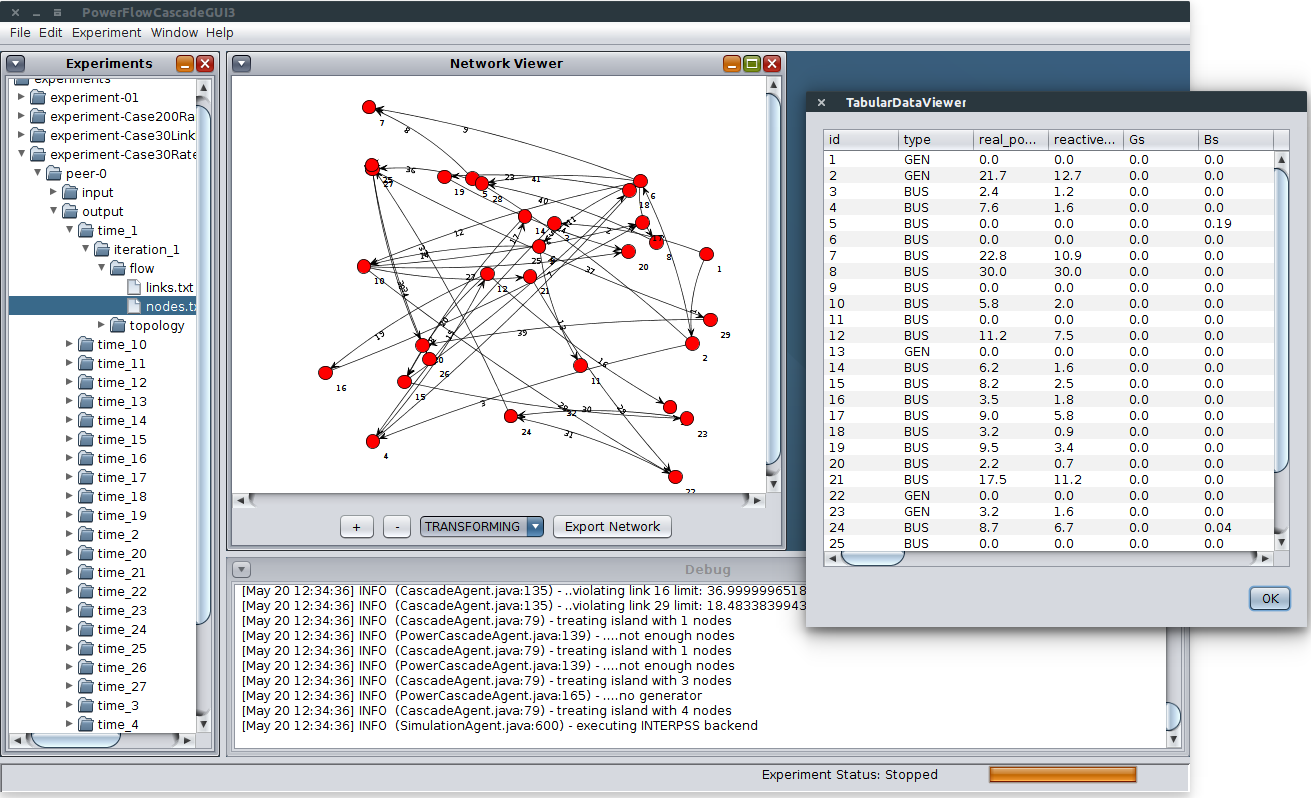
\includegraphics[width=\columnwidth]{GUI/differentFeaturesOfTheGUIVisibleAtOnce.png}
	\caption{}\label{fig:GUI}
\end{subfigure}

\begin{subfigure}[t]{0.45\columnwidth}
	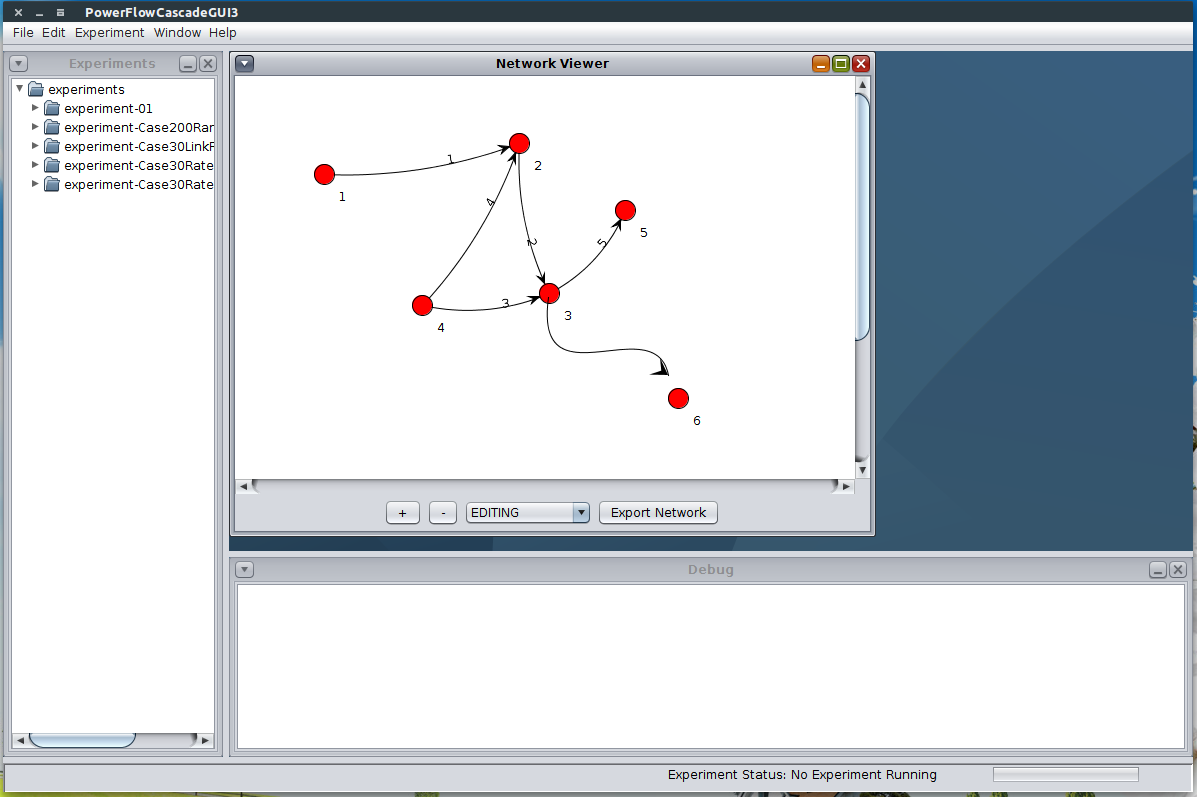
\includegraphics[width=\columnwidth]{GUI/createNetworkFromScratch.png}
	\caption{}\label{fig:GUIcreate1}
\end{subfigure}
\begin{subfigure}[t]{0.45\columnwidth}
	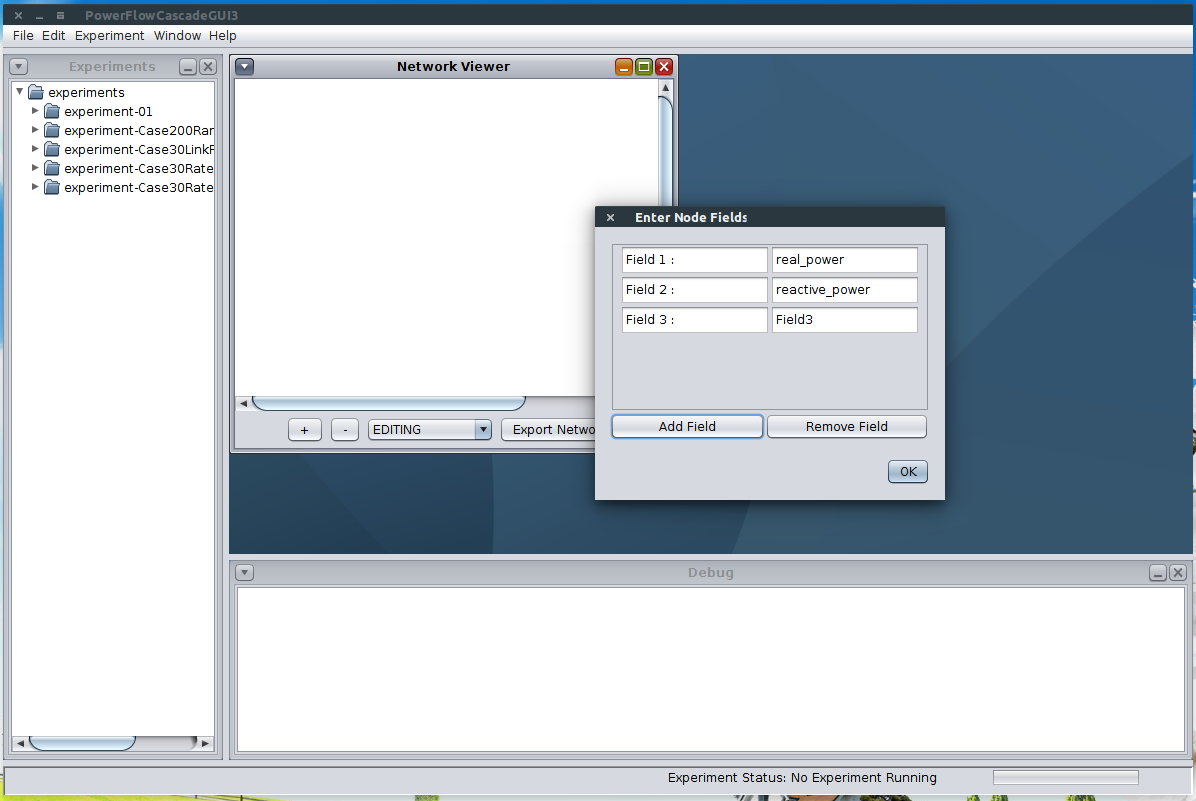
\includegraphics[width=\columnwidth]{GUI/specifyNodeAndLinkFieldsForNetworkCreationFromScratch.png}
	\caption{}\label{fig:GUIcreate2}
\end{subfigure}
\caption{The graphical user interface (a) and how to use it to create a new network (b,c).}
\end{figure}

\subsection{Manual setup}\index{Measurements}\index{Files}\index{Application}\label{sec:Simulation_Measurements}
If the application one wants to use is already implemented and the goal is to only execute it with own parameters and input data, this section explains how to do so. In this case the algorithm and the types of performed measurements cannot be changed. But still several things can be adjusted in order to run different experiments: The name of the experiment, for how many time steps to run the simulation, the \backend{} to use, any event to be executed at any time and when to reload a network from files or when not to do so. In order to run a simulation, one should follow these steps: 

\begin{itemize}
	\item Create a folder in experiments for this simulation, and put an input folder. Let’s call our simulation “test”, then we would need to create experiments/experiment-test/input
	\item Put all the necessary input files there
	\begin{itemize}
		\item events.txt
		\item \backendParametersFile{}
		\item time\_1/topology/nodes.txt and links.txt
		\item time\_1/flow/nodes.txt and links.txt
		\item More time folders in the same structure as time\_1, if we want to load a different new network configuration at a later time step. If no input files are provided, the simulation continues to use the data from the last simulation step. For more details on the input files and how to format them, see section \ref{subsec:config_files}.
	\end{itemize}
	\item Optionally put events to be executed in events.txt. Here it is also possible to define the reloading of the first input folder by putting at time n, where this should happen:
	\begin{lstlisting}
		n,system,-,-,reload,1
	\end{lstlisting}
	\item  Create a new class (e.g. testExperiment.java to run the Power\CascadeAgent{}.java application) in the following way:
\end{itemize}
	\begin{lstlisting}[frame=single] 
import application.PowerCascadeAgent;
import applications.BenchmarkLogReplayer;
import protopeer.Experiment;
import protopeer.Peer;
import protopeer.PeerFactory;
import protopeer.SimulatedExperiment;
import protopeer.util.quantities.Time;

public class testExperiment extends SimulatedExperiment{    

    // define a name for this experiment
    private final static String expName="test";    
    private static String experimentID="experiment-"+expName;
    
    // time steps including bootstrap time
    private final static int runDuration=10;

    // number of networks
    private final static int N=1;
	    
    // other simulation Parameters
    private final static int bootstrapTime=2000;
    private final static int runTime=1000;
    
    public static void main(String[] args) {
        Experiment.initEnvironment();
        testExperiment test = new testExperiment();
        test.init();
        
        // create the instance of PowerCascadeAgent, 
        // contained in a Protopeer peer
        PeerFactory peerFactory=new PeerFactory() {
          public Peer createPeer(int peerIndex, Experiment experiment){
              Peer newPeer = new Peer(peerIndex);
              // add the simulation agent
              newPeer.addPeerlet(new PowerCascadeAgent(experimentID));
              // add the agent managing the simulation steps
              newPeer.addPeerlet(new TimeSteppingAgent(
                  Time.inMilliseconds(bootstrapTime),
                  Time.inMilliseconds(runTime)));
              // add the backend, 
              // in this case Power Simulation with InterPSS
              newPeer.addPeerlet(new InterpssFlowDomainAgent());
              return newPeer;
            }
        };
        test.initPeers(0,N,peerFactory);
        test.startPeers(0,N);

        // run the simulation
        test.runSimulation(Time.inSeconds(runDuration));

        // analyze measurements
        BenchmarkLogReplayer replayer =
        new BenchmarkLogReplayer(expName, 0, 1000);
}
	\end{lstlisting}
First notice, that our testExperiment class extends SimulatedExperiment, which is a Protopeer class (section \ref{subsec:protopeer}) providing useful functionality like time and measurements. Then it is necessary to assign to experimentID the same name as the input directory is called, in order for the experiment to find the files. The runDuration variable defines for how many time steps the simulation will run, including the bootstrap time, which is used to initialize the experiment. Defining the bootstrapTime as 2000 ms and the runTime as 1000 ms, a runDuration of 10 corresponds to 8 simulation steps. So in general: \textit{runDuration = bootstrapTime/runTime + number of actual simulation steps}. 

Different agents, encapsulating separate functionality, have to be added. For more details see section \ref{sec:agents}. Different configurations are possible, however at least three agents are necessary, one from each of the following categories:
\begin{enumerate}
	\item A \MainAgent{}, which is extended to different functionality, for example \BenchmarkAgent{} for measurements or the Power\CascadeAgent{} for running cascade simulations in power networks.
	\item \TimeAgent, for a simulation on one single network this is the \TimeSteppingAgent{} as in the above example. For interdependent simulations between multiple networks the \SimpleCommunicationAgent{} should be added, as explained in more detail in section \ref{sec:agents}.
	\item A \DomainAgent, for example \InterpssDomainAgent{} or \MatpowerDomainAgent{} (requiring a Matlab installation) in the case of a power network simulation.
\end{enumerate}

The only thing left to do, is to initialize the peer we just set up, and finally executing it with test.runSimulation(...).

\subsection{Measurements}
All the measurement results are saved to a binary file in peerlets-log/experimentID/peer-0, from where it can be loaded after the simulation finished to compute, display and output measurement results. This functinality is provided by the SFINA Flow Monitor package, which one the one hand logs (BenchmarkSimulationAgent) and processes the logged information (\BenchmarkLogReplayer{}). The \BenchmarkLogReplayer{} shows the processed results in a table in the console and log files, and also writes the values to files in the folder results/experimentID for further processing.

To see what is going on during the simulation, logging is useful. For this first it is necessary to make sure in conf/log4j.properties the line “log4j.rootLogger=info, I, stdout” isn’t commented out. This will show information during the simulation and also the measurement output in the console and in the file log/info.log. To get a finer grained output, uncomment “log4j.rootLogger=debug, D, stdout” in the same .properties file.

All the measurement classes are in www.github.com/SFINA/Flow-Monitor.


\section{Existing Applications}\label{sec:existing_apps}

\subsection{Cascading Simulations in Power Grids}\index{Agent!Power\CascadeAgent{}}
This is an example of a more sophisticated application. As can be seen in figure \ref{fig:apps} there are two levels:
\begin{enumerate}
	\item Cascade Agent: Implementing a general cascade algorithm with a method that checks the links for overloads (i.e. the flow in the link exceeding its capacity). It implements (overrides) the runFlowAnalysis() method of the SimulationAgent, but also introduces a new method, namely flowConvergenceStrategy() which is an intermediary step before calling the \backend{} to calculate the power flow in the network. This allows a very flexible implementation of different (\domain{} dependent) necessary adjustments. This is exactly what is implemented by the Power Cascade Agent, which brings us to the next point.
	\item The Power Cascade Agent mainly implements flowConvergenceStrategy() from the Cascade Agent. It first checks if the current island just consists of one isolated node, returning directly non-convergence (i.e. blackout) in this case. Then it checks if there is a generator present in the island, because without power supply the island is also blacked out. Furthermore it tries to improve convergence, i.e. finding a stable solution for the power flowing in the network, by adjusting load and generation. Finally the Power Cascade Agent implements some more measurements, for example the number of islands and isolated nodes and the power demand which cannot be served (load loss).
\end{enumerate}
The code is in www.github.com/SFINA/Cascade.

\subsection{Smart transformers for mitigation of cascading failures}
For preventing cascading failures in power grids smart transformers can be used (Pournaras, Espejo-Uribe, \textit{Self-Repairable Smart Grids via Online Coordination of Smart Transformers}, IEEE Transactions on Industrial Informatics, 2016). This is implemented in the PowerMitigationAgent which extends the PowerCascadeAgent and introduces these smart transformers into the network. It overrides mitigateOverload() method defined in PowerCascadeAgent (see above), where it adds the sensitivity factors of each transformer, initial flow of each link (in percent) and initial angle to some links, which are defined to be transformers by the input files. The optimization problems presented in above mentioned paper are modeled and solved with the Gurobi Java API and Gurobi 6.5.2, respectively. The code can be found in www.github.com/SFINA/Smart-Transformers.

\subsection{Disaster spreading in complex networks}
\todo[inline]{disaster spread description missing}


%----------------------------------------------------------------------------------------
%	CHAPTER ARCHITECTURE
%----------------------------------------------------------------------------------------

\chapter{Architecture}
\label{ch:architecture}

For running experiments which are already implemented it is only necessary to understand the file system and the concept of events. For a deeper understanding and to implement own applications, the information about the flow network, the different agents and Protopeer will come in handy. 

%------------------------------------------------

\section{File System}\index{Files}\label{sec:file_system}
The SFINA file system allows easy input and output of all the network information needed for the simulation. Every agent has its own file system, where for each experiment a new directory has to be created and provided with input data and configuration files. The simulation automatically performs the output in the same format as the input, i.e. one folder per time step, however extended by finer grained simulation steps (iterations). The notion of time and iterations is explained in the following paragraphs. The file system is illustrated by figure \ref{fig:file_system}, where input files or folders that show a solid contour have to be provided, the dashed ones are optional, as explained in more detail below.

\begin{figure}[h]
\centering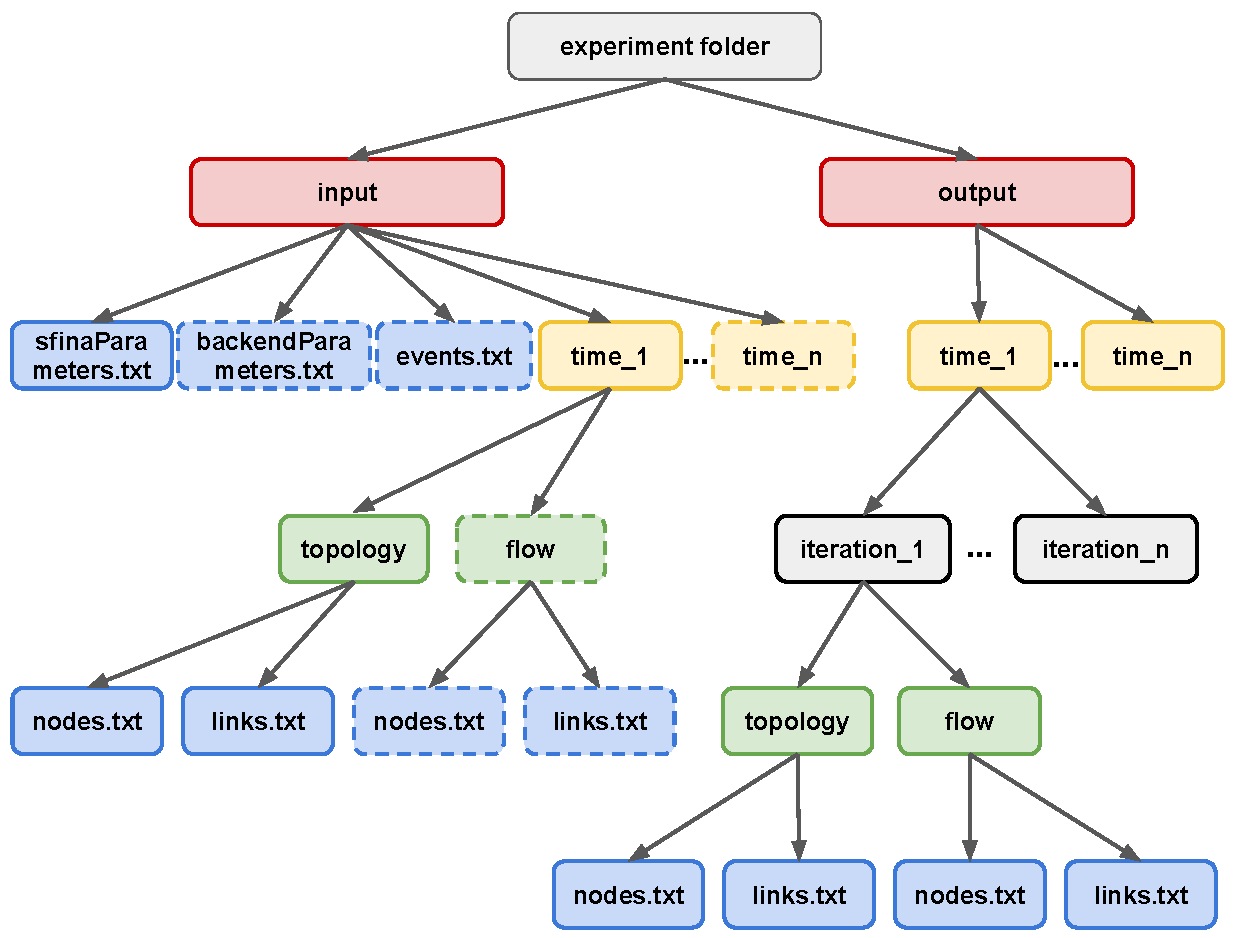
\includegraphics[width=0.95\textwidth]{file_system.pdf}
\caption{Visualisation of the SFINA file system. In input, files/folders with dashed boxes don't have to be provided. The output folder is created automatically.}
\label{fig:file_system}
\end{figure}

\subsection{Location of the files}\index{Files!Location}
Each experiment is assigned a string identifier, defined when running experiments (section \ref{sec:Simulation_Measurements}). The input files of an experiment with the identifier “someExperiment” have to placed in the folder experiments/someExperiment, where “someExperiment” can be any string.

\subsection{Configuration files}\index{Files!Configuration files}\index{Domain}\index{\Backend{}}\index{Events}\label{subsec:config_files}
Two configuration files are part of an experiment, providing settings for the currently used \backend{} (\backendParametersFile{}) and defining events to be automatically executed (events.txt). The \backend{} parameter file doesn’t have to be provided (i.e. will not result in an error), however depending on the \backend{} certain parameters might be necessary. This is for example the case of AC or DC in the power \domain{}. The event file injects scheduled events to be executed during runtime and can be provided, but the simulation will also run without it. 

\textbf{The \backendparameters{} file} is specified in the format “name=value”. The currently available settings are summarized in table \ref{table:params}.

\begin{table}[h]
\centering
\begin{tabular}{|l| l| l|}
\hline
\rowcolor{Gray}
File & Name & Possible values\\
\hline
\multirow{2}{*}{\parbox{4cm}{\backendParametersFile{} (power \domain{})} } & flowType & AC, DC \\ 
\cline{2-3} & toleranceParameter & value of type double \\ \hline
\backendParametersFile{} (disaster spread \domain{}) & - & - \\ \hline
\end{tabular}
\label{table:params}
\caption{Parameters that can be specified in the parameter files. Currently no \backendParametersFile{} for disaster\textunderscore spread \domain{} are necessary.}
\end{table}

\textbf{The events file} has the following format, defining one event per line with comma separated values:

\begin{lstlisting}[frame=single] 
time,feature,component,id,parameter,value
2,topology,link,10,status,0
3,flow,link,9,resistance,0.1
3,system,-,-,reload,1
...
\end{lstlisting}

For a more detailed explanation how events work and which ones are available, see  section \ref{sec:events}. The events are loaded at the beginning, but each of them is executed at the time specified in the first column. It allows to define certain important events before running the experiment and without the need to modify the code. 

\subsection{Network data}\index{Files!Network data}\index{Flow}\index{Topology}
Each time\_n folder in input as well as in output/iteration\_m contains the full network data, separated into general topological information and \domain{} specific flow information. All the output files are generated automatically, so only the input folder has to be provided in order to run an experiment. A folder time\_n in input is loaded at time step n and replaces all the network information (both topological and flow) from earlier times. At least the time\_1 folder with data has to be provided in order for the experiment to have sufficient data to run. If a folder at any time step is present, it will automatically be loaded, discarding the data from before and replacing it with the new one. On the other hand it will continue with the information from the time step before if no folder for the current time is present.

\paragraph{Topological data} The topological data provides the nodes/links with a unique ID, which can be any string, and a status attribute which specifies if it is active or not. In the latter case the simulation treats it as if it was not present, but it can be activated during runtime for example by events. Links are directed, which can be specified by the IDs of the nodes where it starts and ends. An undirected link can be simulated by creating two links, one in each direction. The formatting of the files is shown in figure \ref{fig:input_files}.

\begin{figure}[!h]
\centering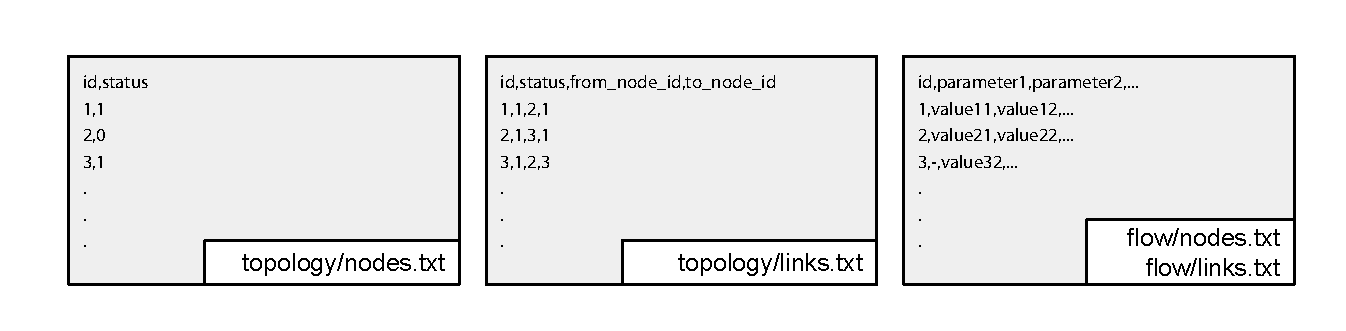
\includegraphics[width=0.98\textwidth]{input_files.pdf}
\caption{Format of topology and flow input files.}
\label{fig:input_files}
\end{figure}

\paragraph{Flow data} The flow data is very flexible and has the same format for both nodes and links, as shown in figure \ref{fig:input_files}. For each node/link information can be loaded that is needed for the flow simulation of the current \domain{}. For example in the power \domain{} this might be the generation output or load of a node or the resistance of a link. Similarly, for disaster\textunderscore spread \domain{}, flow data for links could be connection strength and time delay whereas for nodes this could be initial recovery rate or tolerance of the node. The values are then stored in the nodes and links of the ID specified in the first column.

The flow data is \domain{} specific and therefore has to be defined seperately for each one. Currently this is the case for the power and disaster\textunderscore spread \domain{s}, other \domain{s} are not supported yet.

In the most general case of purely topological networks, the flow data could be used to assign weights to the links or nodes. However in general it is not necessary to provide flow input files, in that case a topological network with no further attributes is generated.

Some nodes or links might be of a different kind than others, making it necessary to assign certain values to them but not to the others. In the power \domain{} this is for example the case for nodes that generate power, which additionally need among others the power generation output information. In this case a dash (-) can be used to exclude this information from all other nodes as seen for value31 in the example above, it will be ignored during loading. 

\subsection{Manually loading network data}\index{Loading}\index{Files!Loading}
As explained in section \ref{sec:simu_agent} about the \mainagent, at the beginning of each time step, the corresponding input data is automatically loaded, if provided by the user. It is however also possible to initiate data loading manually, by calling the method loadData(time), where “time” is a string to be replaced with the time matching the input folder time to be loaded. It is also possible to trigger this “reload” of the time x input at time y by an event, as explained further below.

\subsection{Changing the file system structure}
The structure of the file system and names of folders outlined above is defined in a configuration file, which is loaded at bootstraping of the \mainagent{} (section \ref{sec:simu_agent}). It is placed in the folder conf/fileSystem.conf. Besides the names of all the folders and parameter files, it also defines the column separator and the string which is used for excluding data for some of the nodes/links (missingValue) in the input data files, as explained above. These values can be changed, which is however not recommended.

%------------------------------------------------

\section{Events}\index{Events}\label{sec:events}
Events are designed for making changes to the simulation or to the network structure during runtime. They can be used in two ways:
\begin{enumerate}
	\item Specified in events.txt to be loaded at the beginning and executed automatically at their specified time. 
	\item Written in the code of applications in order to change parameters “online”.
\end{enumerate}

An event is defined by six parameters, specifying what action is to be executed at which time step. An overview of these parameters is given with the following table:
\begin{table}[h]
	\centering
	\begin{tabular}{|l| l|l|l | l| l|}
	\hline
	\rowcolor{Gray}
	Parameter & \multicolumn{5}{l|}{Value/Description}\\
	\hline
	\textbf{time} & \multicolumn{5}{l|}{When the event is executed} \\ \hline
	\textbf{feature} & \multicolumn{2}{l|}{topology} & \multicolumn{2}{l|}{flow} & system \\ \hline
	\textbf{component} & node & link & node & link & n/a (placeholder '-') \\ \hline
	\textbf{id} & \multicolumn{4}{l|}{id of the link/node whose information is changed} & n/a (placeholder '-') \\
	\hline
	\textbf{parameter} & status & \multicolumn{1}{p{2.5cm}|}{\begin{itemize}[leftmargin=*,label={-}]
			\item status
			\item start node id
			\item end node id
		\end{itemize}} & \multicolumn{2}{p{4.5cm}|}{Any flow information which was loaded or added} & \multicolumn{1}{p{2.5cm}|}{\begin{itemize}[leftmargin=*,label={-}]
		\item reload
		\item ...
	\end{itemize}}\\
	\hline
	\textbf{value} & 0,1 & \multicolumn{1}{p{2.5cm}|}{\begin{itemize}[leftmargin=*,label={-}]
			\item 0,1
			\item new node id
			\item new node id
		\end{itemize}} & \multicolumn{2}{p{4.5cm}|}{New value} & \multicolumn{1}{p{3cm}|}{\begin{itemize}[leftmargin=*,label={-}]
		\item Time from which input data should be reloaded
		\item ...
	\end{itemize}}\\
	\hline	
	\end{tabular}
	\caption{Summary of currently available events and how to define them.}
	\label{table:events}
\end{table}

\subsection{Using events.txt}
Each line in the events configuration file defines one event, with comma separated entries for each of the six categories introduced above. As a general rule, the entries should correspond to the same strings which are also used in the other files, namely \backendParametersFile{} and the topology and flow data files. For example in the power \domain{} if the goal is to change the resistance of a specific link with id 9 at time 3, it would be:
\begin{lstlisting}
time,feature,component,id,parameter,value
3,flow,link,9,resistance,0.1
\end{lstlisting}
In the case of a system parameter change, component and ID are not applicable. In this case, just put a dash (-) instead. For example to reload data at time 10 form input folder time\_1:
\begin{lstlisting}
time,feature,component,id,parameter,value
10,system,-,-,reload,1
\end{lstlisting}
See section \ref{sec:file_system} about the file system for more details.

\subsection{Using events in an application}
The same categories are used to define events in the code, however instead of strings the appropriate Enum types are used. The constructor of the Event class takes as arguments:
\begin{lstlisting}
Event(int time, 
	EventType eventType, 
	NetworkComponent networkComponent, 
	String componentID, 
	Enum parameter, 
	Object value)
\end{lstlisting}
Let’s look at an example, which deactivates link 20 at time step 10:
\begin{lstlisting}
Event event = new Event(
	10,
	EventType.TOPOLOGY,
	NetworkComponent.LINK,
	"20",
	LinkState.STATUS,
	false);
queueEvent(event);
\end{lstlisting}
The last command schedules the events for execution at their defined time step.
%------------------------------------------------

\section{Flow Network}\index{Flow Network}\label{sec:flow_net}
The flow network is an object containing all the nodes and links and providing several useful methods, explained in the following. 

\subsection{Activation status and connectivity}\index{Activated}\index{Connected}\index{Islands}
First of all the flow network takes care of adding nodes/links to and removing them from the network and updating the network topology accordingly. The two basic topological properties a node/link can have are
\begin{enumerate}
	\item isConnected(): A node which has (activated) links attached, or a link that has both (activated) start and end node, is connected.
	\item isActivated(): A node/link that is functional, is activated. Deactivating a node, will not deactivate the attached links, but just disconnect them. Likewise, a disconnected node is still activated.
\end{enumerate}

Once the network is loaded, it is possible to activate/deactivate nodes/links in the network, which will include/exclude them from any computation but will not remove them entirely. This way they can be used again later on. The nodes and links also keep track of their connectivitiy, i.e. if any other objects are connected or not. This information can be retrieved by the method isConnected().

An important method in the network is computeIslands() which extracts disconnected components from the topology of the network and returns them as an ArrayList containing a new flow network for each island. It takes all activated nodes/links into account, as can be seen in figure \ref{fig:flow_net}.

\begin{figure}[!h]
\centering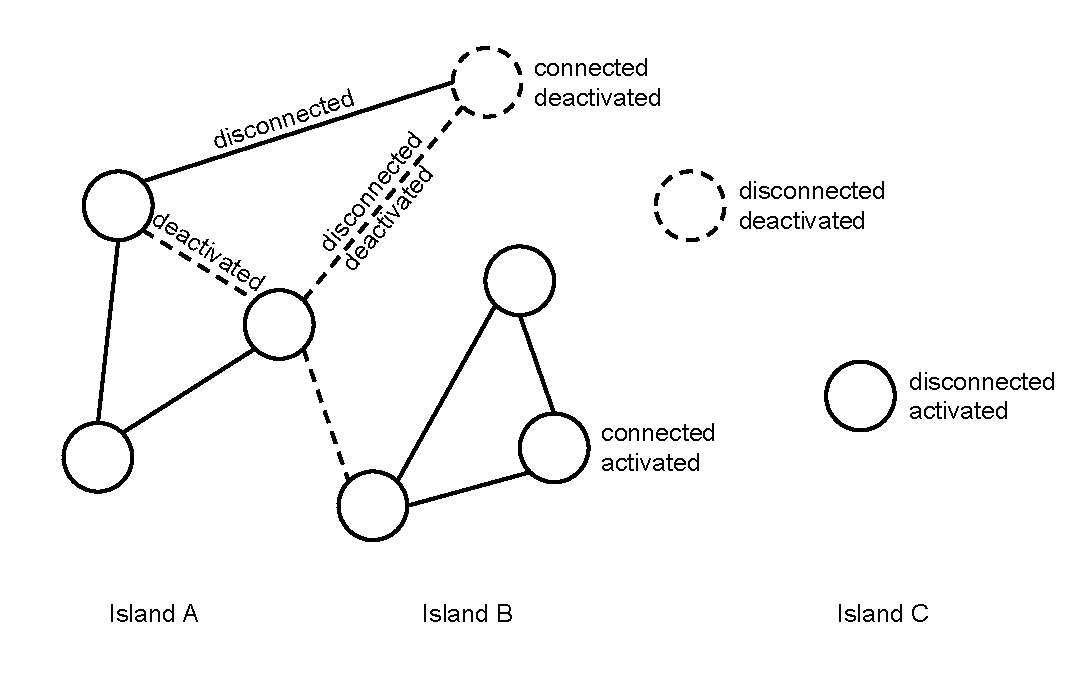
\includegraphics[width=0.95\textwidth]{flow_network.pdf}
\caption{Illustration of the connectivity and activation status of nodes and links, and how they affect the computation of disconnected compontents (i.e. islands).}
\label{fig:flow_net}
\end{figure}

\subsection{Metrics}\index{Metrics}
Furthermore the flow network provides some useful methods to calculate metrics like degree distribution, clustering coefficient or to find the shortest path between two nodes. Some of these methods use the openly available \href{http://jgrapht.org/}{JGraphT library}. A more detailed list can be found in the method summary in section \ref{sec:net_methods}.

\subsection{Flow and capacity}\index{Flow}\index{Capacity}
The flow network provides a flexible way to define the flow and capacity, meaning which physical quantities (contained in the nodes and links) is the measure of flow or how much flow a node/link can support. Use setLinkFlowType(...) and setLinkCapacityType(...) and for the nodes respectively for this purpose. This is done in the setFlowParameters() method in the \mainagent, where each \domain{} has its default settings. When developing a new application, the developer is expected to check these. Default values are summarized in the following table.
\begin{table}[h]
	\centering
	\begin{tabular}{|l| p{2.5cm}| p{2.5cm}|l|l|}
	\hline
	\rowcolor{Gray}
	\Domain{} & Link flow type & Node flow type & Link capacity type & Node capacity type\\
	\hline
	Power & Real power flow from & Voltage magnitude & C rating & Max. voltage\\
	\hline
	disaster spread &\dots &\dots &\dots &\\
	\hline
	\dots &&&&\\
	\hline
	\end{tabular}
	\caption{Default values for capacity and flow for the different \domain{s}.}
	\label{table:flow_capacity}
\end{table}

\subsection{Accessing the flow network and its values}\index{Flow Network}
Some hints which might come in handy when writing applications:
\begin{enumerate}
	\item When writing an application which extends the SimulationAgent, the current flow network can always be retrieved by the method getFlowNetwork().
	\item To add new flow information to a node or link, use the .addProperty(...) method.
	\item To get or change the flow information already contained in the nodes or links, use the .getProperty(...) or .replacePropertyElement(...) method respectively. The former requires casting the return value to the correct type.
\end{enumerate}

Here you see these in action, doubling the real power demand of node 15 in the current flow network:
\begin{lstlisting}[frame=single] 
FlowNetwork net = getFlowNetwork();
Node someNode = net.getNode(15); // node having ID 15
double pwr = 
	(Double)someNode.getProperty(PowerNodeState.POWER_DEMAND_REAL);
someNode.replacePropertyElement(PowerNodeState.POWER_DEMAND_REAL,pwr*2);
\end{lstlisting}

A summary of methods can be found in the appendix (section \ref{sec:net_methods}).

\section{Time and iteration}\index{Iterations}\index{time}
A SFINA simulation is clocked by time units, which are executed sequentially. At the beginning of each time unit new input files (toplogy, flow and events) can be provided to the simulation.

During each time step several simulation iterations can be performed, depending on the logic implemented in the \TimeAgent{}. One can for example decide to perform another simulation iteration in the current time step, if the simulation did not converge in the previous iteration. By default the user triggers another iteration by calling queueEvent(event) with an event defined for the current time step. Before advancing to the next time step, the event queue is checked for remaining events and executes new iterations as long as it is not empty (for the current time).

\begin{figure}[!h]
\centering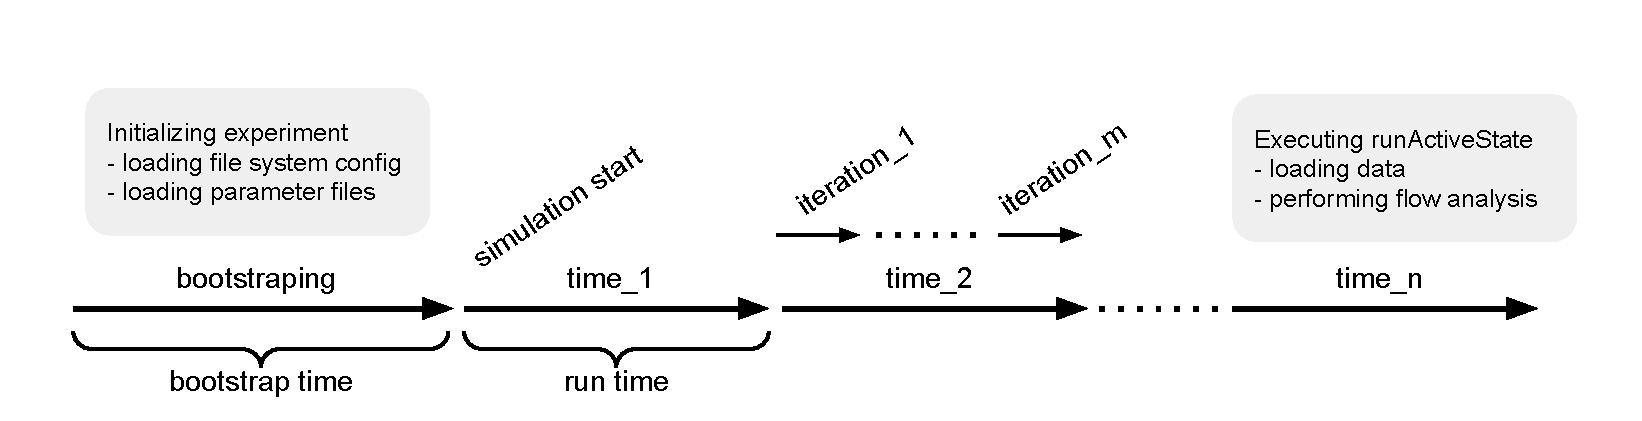
\includegraphics[width=0.95\textwidth]{time_iterations.pdf}
\caption{Time steps and iterations performed by the active state.}
\label{fig:time_iter}
\end{figure}


%------------------------------------------------
\section{Protopeer Toolkit (redo, maybe split in part here and appendix)}\index{Protopeer}\label{subsec:protopeer}
\todo{work over protopeer section}SFINA makes use of the Protopeer Toolkit which was developed at EPFL university Lausanne to provide a framework for peer to peer distributed experiments (\href{http://infoscience.epfl.ch/record/128659/files/protopeer_demo.pdf}{paper}). It provides useful basic functionality like time based events and measurement methods. Another important concept is peers and peerlets, which allow a fully decentralized deployment. A peer is an independent simulation instance, which can communicate over the network with other peers. Every peer can contain several peerlets, which allow to further split up a peer in seperate simulations. % Currently experiments conducted with SFINA initialize just one peer with one peerlet. However this potentially allows for a very flexible use of the SFINA framework in the future.
%------------------------------------------------



%----------------------------------------------------------------------------------------
\chapter{Agents}\index{agent, peerlet}\label{sec:agents}
%----------------------------------------------------------------------------------------
The SFINA framework utilizes the protopeer library, which allows through its concepts of peers and peerlets to encapsulate different functionality separatetely. See section \ref{subsec:protopeer} for an introduction to protopeer. Each simulation is configured as a peer (see chapter \ref{ch:introduction} for an example). When creating an experiment, different agents, which implement the Peerlet interface and encapsulate separate functionality, have to be added to the peer. For example when running an experiment with interdependent networks, one can simply configure a different peer for each network. In this case one needs to add a \CommunicationAgent{} and \NegotiatorAgent{} instead of the \TimeAgent{} to the peer.\\
The following agents have to be added to the peer as peerlets when setting up an experiment (see section \ref{sec:Simulation_Measurements}) In brackets we note in which setup (single/ interdependent network) the agent \textbf{must} be added:
\begin{enumerate}
	\item \MainAgent \tabto{4cm} (both)
	\item \DomainAgent \tabto{4cm} (both)
	\item \TimeAgent \tabto{4cm} (single network)
	\item \CommunicationAgent  \tabto{4cm} (interdependent)
	\item \NegotiatorAgent \tabto{4cm} (interdependent)
\end{enumerate}
The different agents allow a SFINA experiment to be set up in a modular way. Hence one can easily extend core functionalities of SFINA (see chapter \ref{ch:core_functionality_extension}) or build new applications on top of the framework (see chapter \ref{ch:new_applications}) through replacing some of the agents. The different agents are explained in more detail in the following.

%----------------------------------------------------------------------------------------
\section{Process flow of a basic simulation}
\todo{Best would be to provide a graphic about the process flow}In the following we present the general process flow of a simulation. This is applies to the interdependent and non-interdependent case.
\begin{enumerate}
	\item Initialization:
	\begin{itemize}
		\item All Peers call \textit{init()} on their Agents (Peerlets)
		\item The agents perform necessary initializations
	\end{itemize}
	\item Start:
	\begin{itemize}
		\item Peers call \textit{start()} on all their Agents.
		\item \textit{start()} should only be implemented in the \TimeAgent{}
		\item \TimeAgent{} calls \textit{runBootstrapping()} on the \MainAgent{}
	\end{itemize}
	\item Bootstrap:
	\begin{itemize}
		\item \MainAgent reads necessary parameters from input files, schedules measurements etc.
		\item when finished, \MainAgent{} calls \textit{agentFinishedBootstrap()} on \TimeAgent{}
	\end{itemize}
	\item Start simulation/ Progressing to next time step
	\begin{itemize}
		\item \TimeAgent{} calls \textit{progressToNextTimeStep()} on \MainAgent
		\item \MainAgent{} initializes the first time step.
		\item Afterwards \MainAgent{} calls \textit{agentFinishedActiveState()} on \TimeAgent{}
		\item Then \TimeAgent{} progresses \MainAgent{} to next iteration. In order for this to function, \MainAgent{} has to signal, that it did not converge yet.
	\end{itemize}
	\item Progess of Simulation
	\begin{itemize}
		\item From now on, after each simulation iteration \MainAgent{} calls \textit{agentFinishedActiveState()} on \TimeAgent{}. \TimeAgent{} then decides to 
		\begin{enumerate}[label=(\alph*)]
			\item either perform another simulation iteration through calling \textit{progressToNextIteration()} on \MainAgent{}
			\item or to skip the next iteration (makes sense for interdependent case to synchronise different networks) through calling \textit{skipNextIteration()} on \MainAgent{}
			\item or to progress \MainAgent{} to the next time step through calling \textit{progressToNextTimeStep()}, hence return to the 4th step.
		\end{enumerate}  
	\end{itemize}
\end{enumerate}


\section{Simulation Agent}\index{Agent!Simulation Agent}\label{sec:simu_agent}
At the heart of any simulation is the simulation agent. Applications extend it and can therefore make use of its functionality (see section on adding applications for more detail). The \mainagent{} takes care of performing several tasks which are necessary for any simulation. These include loading and performing output, executing events and calling key methods at every time step. The time evolution of the simulation agent is illustrated by figure \ref{fig:time_iter}. Itself, it provides only barebone functionality and is extended for enabling more complex simulations, for example the
	\begin{enumerate}
		\item FlowMonitor, measuring and logging information during simulation.
		\item \CascadeAgent{} and its extention Power\CascadeAgent{}: Simulating cascading failures due to link and/or node overloads (i.e. capacity < flow). The latter specifically implements strategies and modifications for cascades in power networks.
	\end{enumerate}

\subsubsection{The Active State}\index{Active State}\index{Events}
The runActiveState() method is the main runtime of the \MainAgent{}. After bootstraping, during which the experiment is initialized by loading the configuration files from the experiment folder, the main simulation is orchestrated by the this method. It is executed at every time step automatically and initiates the above mentioned tasks, as depicted in detail in figure \ref{fig:active_state}.

\begin{figure}[!h]
\centering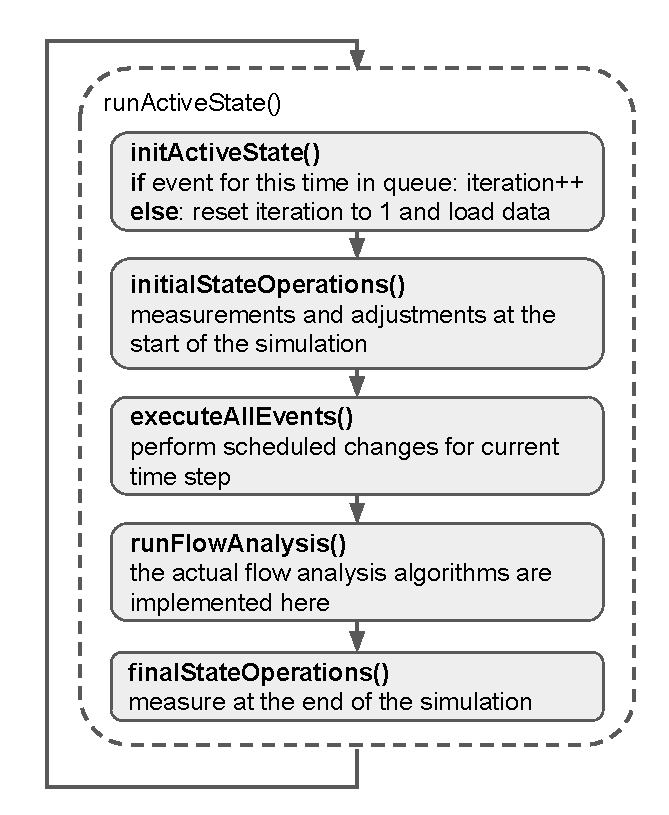
\includegraphics[width=0.6\textwidth]{active_state.pdf}
\caption{Methods executed by the active state in each time step.}
\label{fig:active_state}
\end{figure}

The \MainAgent{} class is providing this minimal but extensible structure, without implementing any specific algorithm on how to perform the flow analysis at each time step. Such algorithms are meant to be implemented in applications by overriding 
\begin{enumerate}
	\item initialStateOperations()
	\item runFlowAnalysis()
	\item finalStateOperations().
\end{enumerate}

In the SimulationAgent, the initialStateOperations and finalStateOperations methods are empty, but can be overridden in applications for more functionality. In runFlowAnalysis() callBackend() is executed to calculate the actual flow distribution in the network. This method can be called as often as necessary, i.e. is up to the developer of an application (see section \ref{sec:apps} on implementing new applications for more detail). 

A new iteration is initiated automatically if there are pending events for the current time step. Also the output of the files is done automatically. 

The two methods initialStateOperations() and finalStateOperations() are especially useful for making measurements before and after the flow analysis. Also this allows to implement measurements, which depend on the state before and after the flow analysis. However, they can also be used to implement additional functionality, especially adjustments to the network at the beginning through events, which are then executed automatically in the executeAllEvents() method (more details in section \ref{sec:Simulation_Measurements} about measurements).

The callBackend() method executes the \backend{}, which is automatically selected according to the FlowDomainAgent chosen in the experiment class. Currently implemented \backend{s} are shown in the followig table.
\begin{table}[h]
	\centering
	\begin{tabular}{|l| l |l|}
	\hline
	\rowcolor{Gray}
	\textbf{\Domain{}}&\textbf{\Backend{}}\\
	\hline
	power & interPSS, Matpower (Matlab required)\\
	\hline
	disaster\_spread & helbingetal\\
	\hline
	\dots & \dots\\
	\hline
	\end{tabular}
	\label{table:backends}
	\caption{Currently integrated \backend{s} to calculate flow in a network.}
\end{table}


%------------------------------------------------
\section{\TimeAgent}\index{Agent!\TimeAgent}\label{sec:time_agent}
Organizes the time steps of the simulation, calls \MainAgent{} when it should simulate the network and gets in turn notified by the \MainAgent{} when it finished its iteration. 
Has to implement the following interface in order to function within the SFINA framework:

\begin{lstlisting}[frame=single] 
/**
* A TimeStepping Agent needs to implement this interface.
* @author mcb
*/
public interface TimeSteppingAgentInterface {

/**
* SimulationAgent can notify the TimeSteppingAgent 
* that it finished its Step
* 
*/
public void agentFinishedActiveState();

/**
* SimulationAgent can notify the TimeSteppingAgent 
* that it finished its Bootstrap
*/
public void agentFinishedBootStrap();

/**
* Returns the current Simulation Time.
* @return 
*/
public int getSimulationTime(); 
}
\end{lstlisting}

The following default implementation exist:
	\begin{enumerate}
		\item \TimeSteppingAgent{}: Simulates a single network, advances \MainAgent{} directly when its ready.
	\end{enumerate}
	
%------------------------------------------------
\subsection{\CommunicationAgent}\index{Communication Agent! \CommunicationAgent}\label{sec:communication_agent}	
Abstract class which extends \TimeSteppingAgent{}. Thus it has the same core responsibility as \TimeAgent.
In addition \CommunicationAgent{} handles the communication between interdependent networks and is responsible for the order of execution of Simulation iterations. The following two extensions exist:
\begin{enumerate}
	\item \InterdependentCommunicationAgent{}: Allows for multiple networks to be connected, thus manages their synchronization and exchange of information. The execution logic is of a parallel nature: Each iteration of all networks happens in parallel, after which the networks update each other. 
	\item \TokenCommunicationAgent{}: Organizes interdependent networks, but executes them in a sequential rather than parallel order. Hence i.e. iteration 1 of network 1 happens before iteration 1 of network 2.
\end{enumerate}

For more information on interdependent network simulations, see section \ref{sec:interdep}.
	
	
%------------------------------------------------
\section{\DomainAgent}\index{Agent!\DomainAgent}\label{sec:domain_agent}
Provides the simulation of a distribution of flows in the network for given input data. It also handles the translation of the input file values which are specific to each \domain{} during input and output. In the case of power simulations this can be \InterpssDomainAgent{} or \MatpowerDomainAgent{}.


%------------------------------------------------
\section{\NegotiatorAgent}\index{Agent!\NegotiatorAgent}\label{sec:negotiator_agent}
Responsible to resolve event conflicts in interdependent network simulations: If an interdependent link tries to change the same property of a specific link or node, then the negotiator decides how to reconcile them.


%----------------------------------------------------------------------------------------
%	CHAPTER Interdependent
%----------------------------------------------------------------------------------------

\chapter{Interdependent Network Simulations}\index{interdependent}\label{sec:interdep}
In the following we will show how to set up a basic interdependent network simulation and explain the core ingredient in detail, namely the \CommunicationAgent{}.
\section{The \CommunicationAgent}
\todo[inline]{complete communication agent section}

\section{Simulation of an interdependent experiment}
Equipped with the knowledge of the setup of a single network experiment (see section TBD) and the functioning of the \CommunicationAgent{} it will be easy to understand the setup of an interdependent network experiment. 
It namely boils down to the addition/ adjustment of the bold parts in the following experiment file.
Instead of a \TimeAgent a \CommunicationAgent{} and a \NegotiatorAgent have to be added to the experiment file and the number of networks has to be specified:

\begin{lstlisting}[frame=single] 
public class TestCommunicationAgent_communicationTimeStepping
 extends SimulatedExperiment{
	
	private static final Logger logger =
	 Logger.getLogger(
	 TestCommunicationAgent_communicationTimeStepping.class);
	
	
	private final static String expSeqNum="01";
	private static String experimentID="experiment-"+expSeqNum;
	
	//Simulation Parameters
	private final static int bootstrapTime=2000;
	private final static int runTime=1000;
	private final static int runDuration=6;
\textbf{	private final static int N=3;}
	
	public static void main(String[] args) {
		Experiment.initEnvironment();
		TestCommunicationAgent_communicationTimeStepping test = 
		new TestCommunicationAgent_communicationTimeStepping();
		test.init();
		
		PeerFactory peerFactory=new PeerFactory() {
			public Peer createPeer(int peerIndex, 
			Experiment experiment) {
				Peer newPeer = new Peer(peerIndex);
				newPeer.addPeerlet(new SimulationAgent(
				experimentID));
				//NECESSARY HELPER AGENTS
			\textbf{	newPeer.addPeerlet(
			new InterdependentCommunicationAgent(
			Time.inMilliseconds(bootstrapTime),
				Time.inMilliseconds(runTime),N));}
				newPeer.addPeerlet(
				new InterpssFlowDomainAgent());
				newPeer.addPeerlet(
				new PowerEventNegotiatorAgent());
				return newPeer;
			}
		};
		test.initPeers(0,N,peerFactory);
		test.startPeers(0,N);
		
		//run the simulation
		test.runSimulation(Time.inSeconds(runDuration));
		
	}
\end{lstlisting}

In addition to the small changes, the user needs to provide the usual topology and flow information in the same way as he or she did in the singe network case.




%----------------------------------------------------------------------------------------

%----------------------------------------------------------------------------------------
%	PART FOR DEVs
%----------------------------------------------------------------------------------------

\part{For developers}

%----------------------------------------------------------------------------------------
%	CHAPTER CORE FUNCTIONALITY
%----------------------------------------------------------------------------------------

\chapter{Core functionality extension}
\label{ch:core_functionality_extension}
The way to go in order to extend the core functionality of SFINA is to replace agents with own implementations. 
This can be either done through extending an existing version or to implement the correct agent interface.

For adding new applications on top of the SFINA framework one has to extend the \MainAgent or implement its interface, which is described in chapter \ref{ch:new_applications}.


In the following we will outline the main steps to implement own versions of the different SFINA (core) agents.

\section{Backend Calculation: \DomainAgent}\index{\Backend{}}\index{\Backend{} !Interpss}\index{\Backend{} !Matpower}\index{\Backend{} !Interface}\label{sec:backend}
A \Backend{} is a software module that implements algorithms for the calculation of the flow in the network for given parameters. Often simulation software already exist for various \domain{s}, for example MATPOWER or InterPSS to perform power flow analysis. Three ways to implement new \backend{s}:
\begin{enumerate}
	\item Implementing the flow calculation from scratch, using the SFINA data stored in the flow network, nodes and links. This is the most straight-forward way, and definitely the cleanest, resulting in a fully integrated \backend{}. Depending on the complexity however, this can be quite a big task.
	\item Integrate an existing \backend{} which was written in Java. This was done for example for InterPSS. First the SFINA data has to be translated to the new \backend{s} specific format, then its power flow algorithm is called and finally the data is translated back to SFINA. It can be tedious to make sure the data is translated in the correct way, but potentially providing an easy way to integrate a new \backend{}.
	\item Integrate an existing \backend{} written in another language. MATPOWER, which is written in Matlab, was integrated that way. The approach of 2. applies here as well, however on top an interface between Java and the other language has to be developed or integrated. In the Matlab case a package called matlabcontrol written by a third party was used to call Matlab and pass commands to it.
\end{enumerate}

\subsection{Overview of necessary adjustments}
For a \backend{} to work the following classes have to be implemented, however if only a new \backend{} for an already implemented data structure is to be implemented the second and third steps can be omitted.
\begin{enumerate}
	\item An extention of the abstract class \textit{FlowDomainAgent}. This class takes care of the actual simulation. If a third-party \backend{} is used this class translates the SFINA data to the other format, calls it and translates it back. It is then used as a peerlet in the experiment class as described in section \ref{sec:Simulation_Measurements}.
	\item An implementation of the interface \textit{FlowNetworkDataTypesInterface}. This class properly translates the strings from the input files for the loaders. Every flow value of nodes/links (see section \ref{sec:flow_net} for more information) is assigned to an Enum key, which should additionally be specified in a LinkState and NodeState Enum class. 
	\item An implementation of the \textit{\BackendParameterLoader Interface}. This loads the \backendparameters{}, if there are any. This should be rather straightforward. For example in the case of power simulations this loads from the file whether it is an AC or DC simulation. 
\end{enumerate}

The first and second step are explained in more detail in the following sections.

\subsection{FlowDomainAgent}
This abstract class always has to be extended for a new \backend{}. It takes care of the actual flow computation in the network, given the network data. If a third-party \backend{} is used this class translates the SFINA data to the other format, calls it and translates it back. It is then used as a peerlet in the experiment class as described in section \ref{sec:Simulation_Measurements}.

The main method that has to be implemented is 
\begin{lstlisting}[frame=single]
@Override
public boolean flowAnalysis(FlowNetwork net){
// flow simulation goes here    
}
\end{lstlisting}
It does the calculation and returns true if it found a stable solution for the flow distribution in the network (i.e. converged) and false otherwise.

Every node and link has two general fields capacity and flow, which provide an abstraction of the quantitiy flowing through the object and how much of this quantity flow it can withstand before failing. For every \domain{} a value of the node and link flow parameters have to be designated for this purpose, which is done by the method \textit{setFlowParameters}. The easiest is to look at an example, in this case for power flows:
\begin{lstlisting}[frame=single]
@Override
public void setFlowParameters(FlowNetwork flowNetwork){
    flowNetwork.setLinkFlowType(PowerLinkState.POWER_FLOW_FROM_REAL);
    flowNetwork.setNodeFlowType(PowerNodeState.VOLTAGE_MAGNITUDE);
    flowNetwork.setLinkCapacityType(PowerLinkState.RATE_C);
    flowNetwork.setNodeCapacityType(PowerNodeState.VOLTAGE_MAX);
}
\end{lstlisting}

Finally there are two methods to handle \backendparameters{}. A developer can decide if the newly implemented \backend{} needs some user input parameters to run properly. If this is the case a \BackendParameterLoader{} has to be implemented that loads these values into a HashMap and two methods that call this loader and extract the values from the HashMap, as in the following example for power simulations:
\begin{lstlisting}[frame=single]
@Override
public void extractDomainParameters(){
    this.powerFlowType = 
        (PowerFlowType)getDomainParameters()
        .get(PowerBackendParameter.FLOW_TYPE);
    this.toleranceParameter = 
        (Double)getDomainParameters()
        .get(PowerBackendParameter.TOLERANCE_PARAMETER);
}

@Override
public void loadDomainParameters(String backendParamLocation){
    PowerBackendParameterLoader backendParameterLoader = 
        new PowerBackendParameterLoader(
        this.getParameterColumnSeparator()
    );
    this.setDomainParameters(
        backendParameterLoader
        .loadBackendParameters(backendParamLocation)
    );
}
\end{lstlisting}

\subsection{FlowNetworkDataTypesInterface}
To load/write \domain{} specific data from/to files the loaders have to be able to "understand" them. This is the purpose of the FlowNetworkDataTypesInterface. It handles the translation chain 
\begin{enumerate}
	\item Input
	\begin{enumerate}
		\item In the input file the strings in the first line (header) to Enum type LinkState or NodeState variables. This is done by the method \textit{parseNode/LinkStateTypeFromString}.
		\item For each of the following rows (each belonging to a node/link) translate the data strings to double/integer/string/etc variables. This is done by the method \textit{parseNode/LinkValuefromString}.
	\end{enumerate}
	\item Output, the above but in reverse
	\begin{enumerate}
		\item Enum type Link/NodeState $\rightarrow$ strings for the first line of the file. \\ Method \textit{castNode/LinkStateTypeToString}
		\item double/integer/string/etc variables $\rightarrow$ strings, if necessary replacing them by the missing value string (-) if they don't apply to the data column. \\ Method \textit{castNode/LinkStateValueToString}
	\end{enumerate}
\end{enumerate}

As an orientation the implementations for power simulations can be consulted in the PowerFlowNetworkDataTypes class. When implemented correctly this class should allow the data and event loaders to understand your data and load them into the nodes and links so you can use them in the for flow calculations in the new \backend().

%--------------------------------------------- Section TIME AGENT 
\section{Time Stepping: \TimeAgent }
\todo[inline]{complete time stepping agent section}

%--------------------------------------------- Section Communication Agent
\section{Interdependent Communication: \CommunicationAgent{}}
\todo[inline]{complete communication agent section}

%----------------------------------------------------------------------------------------
%	CHAPTER APPLICATIONS
%----------------------------------------------------------------------------------------

\chapterimage{network1.pdf} % Chapter heading image

\chapter{New applications}
\label{ch:new_applications}

\begin{figure}[!ht]
\centering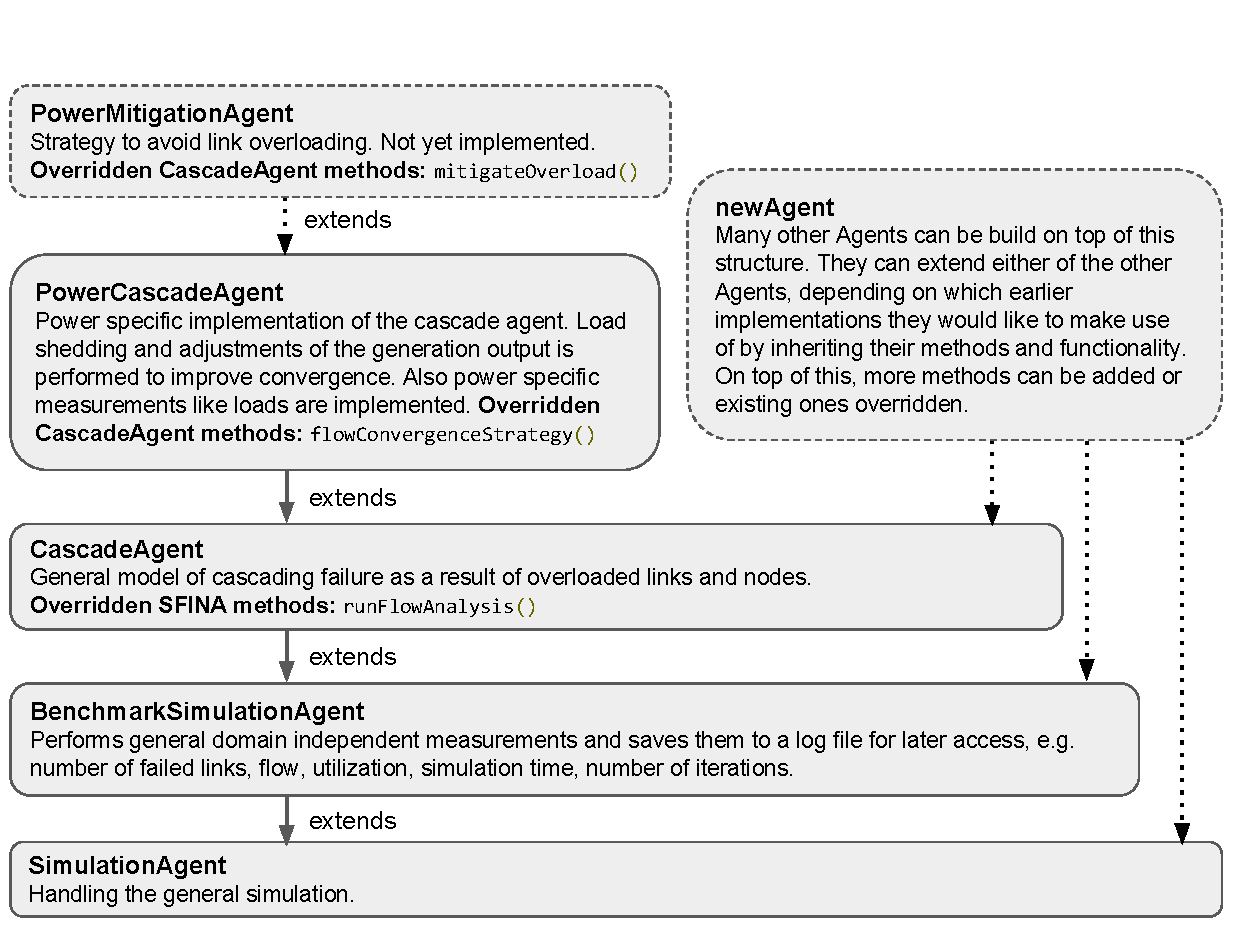
\includegraphics[width=0.95\textwidth]{applications.pdf}
\caption{Architecture of the applications. The ones with dashed solid contours are already implemented, the dashed-contour applications are examples for possible extensions.\todo[inline]{Graphic Needs to be replaced at some point + implement BenchmarkSimulationAgent in a modular way - Use a decorater pattern to allow for runtime additon of benchmark functionality}}
\label{fig:apps}
\end{figure}

\section{Application architecture}\label{sec:apps}
SFINA is designed such that it is flexible and can be easily extended. These extensions can be the implementation of a new application as described in this section, more sophisticated measurements, and more. Currently implemented applications for showcasing the capabilities of the framework as well as for providing basic functionality, are an agent for benchmarking (i.e. making measurements), a model for cascading failures and a specific implementation of the latter for power grid simulations. New applications can be build on top of them in order to make use of their functionalities. If this is not of interest to the developer, totally new applications can be implemented on top of the SFINA core functionality. In any case, whether the SimulationAgent or one of the existing applications are used for the basis of new applications, the capability of Java to extend classes and override methods is used, which will be explained in more detail below. In figure \ref{fig:apps} the current applications are shown, as well as how possible extensions could be realized.

\section{Implementing a new \MainAgent}\index{Agent}
Let’s have a look on how extending one of the existing agent works, taking the example of the \BenchmarkAgent{} Its beginning looks as follows:
\begin{lstlisting}[frame=single]
public class BenchmarkSimulationAgent extends SimulationAgent{
    
    private static final Logger logger = 
    	Logger.getLogger(BenchmarkSimulationAgent.class);
    
    private HashMap<Integer,
    	HashMap<String,HashMap<Metrics,Object>>> temporalLinkMetrics;
    private HashMap<Integer,
    	HashMap<String,HashMap<Metrics,Object>>> temporalNodeMetrics;
    private HashMap<Integer,
    	HashMap<Metrics,Object>> temporalSystemMetrics;
    private long simulationStartTime;
    
    public BenchmarkSimulationAgent(String experimentID, 
            Time bootstrapTime, 
            Time runTime){
        super(experimentID,
                bootstrapTime,
                runTime);
        this.temporalLinkMetrics=new HashMap();
        this.temporalNodeMetrics=new HashMap();
        this.temporalSystemMetrics=new HashMap();
    }
    // Methods
}
\end{lstlisting}
The first thing to notice is the first line, where we define that the \BenchmarkAgent{} extends the \MainAgent{}. This makes all public methods of the latter available for our \BenchmarkAgent{}. Then some variables are defined which are needed for this Agent to store measurement values during runtime. The constructor has to take at least the variables which the SimulationAgent’s constructor needs and passes them on by using the super() method. More variables that are just used for this agent can be added here as well.

Next let’s look at the methods in this agent. Most of them are just new methods necessary for the measurements, for example for initializing the measurement variables in each epoch. The important methods however are the overwritten ones, for example:
\begin{lstlisting}[frame=single]
@Override
public void performInitialStateOperations(){
	// some methods
}
    
@Override
public void performFinalStateOperations(){
	// some methods
}
\end{lstlisting}
They are defined in the \MainAgent{} but don’t have any meaningful implementation there. By overwriting them here, we can “plug in” our own functionality, in this case making measurements before and after the actual flow simulation (see the next section on how to implement measurements for more details).

The \MainAgent{} is the core of every simulation which is not supposed to be changed. Like the methods just introduced, it provides a general structure with methods that can be overwritten, namely:
\begin{enumerate}
	\item public void performInitialStateOperations()
	\item public void runFlowAnalysis()
	\item public void performFinalStateOperations()
	\item public void scheduleMeasurements()
\end{enumerate}

To be precise, these are the only methods of the \MainAgent{} that should be overridden when implementing applications. If your specific application doesn’t seem to fit in this structure, then you maybe didn’t try enough to simplify it, or the current implementation of the \MainAgent{} is not as general as it can be. If this is the case, then you’re welcome to adjust it to your needs and we would be happy to hear about your suggestions and incorporate the changes ourselves.

\subsection{Measurements}\index{Measurements}
In the last chapter we touched on the topic of measurements already by looking at how the \BenchmarkAgent{} is implemented. Here we will explore in more detail how one could implement new measurements, either replacing or by reusing the existing ones. 
Two methods are designed especially to handle measurements:
\begin{enumerate}
	\item public void performInitialStateOperations()
	\item public void performFinalStateOperations()
\end{enumerate}
They are executed before and after the main flow analysis respectively, and allow to save values during the current simulation, for example into one of the measurement variables temporalLinkMetrics, temporalNodeMetrics or temporalSystemMetrics.
To make this more clear, let’s take again the \BenchmarkAgent{} as an example:
\begin{lstlisting}[frame=single]
public void initMeasurementVariables(){
    HashMap<String,HashMap<Metrics,Object>> linkMetrics=new HashMap<>();
    for(Link link:this.getFlowNetwork().getLinks()){
        HashMap<Metrics,Object> metrics=new HashMap<>();
        linkMetrics.put(link.getIndex(), metrics);
    }
    this.getTemporalLinkMetrics().put(
    	this.getSimulationTime(), linkMetrics);
    // initialization of other measurement variables
}        

public void calculateFlow(){
    for(Link link:this.getFlowNetwork().getLinks()){
        double flow=link.getFlow();
        HashMap<Metrics,Object> metrics = 
        this.getTemporalLinkMetrics().get(
        	this.getSimulationTime()).get(link.getIndex());
        metrics.put(
        	Metrics.LINE_FLOW, (link.isActivated()) ? flow : 0.0);
    }
}

@Override
public void performInitialStateOperations(){
    this.initMeasurementVariables();
}
    
@Override
public void performFinalStateOperations(){
    this.calculateFlow();
    // more measurement methods
}
\end{lstlisting}

Here you see the two overridden measurement methods introduced above, which now include new methods performing measurement tasks. The first one just initializes the needed variables to hold the measurement data. The second one gets the current flow through every line and saves it for later use. As long as these measurements are implemented in their own public methods, such as the calculateFlow() method in the above example, they can also be used by other Agents, which further extend the current one.

Measurements in SFINA are using the Protopeer framework (see section \ref{subsec:protopeer} for more details). At the end of each time step, information from the variables introduced above can be saved to a file for later use. This is done in the method scheduleMeasurements() by using log.log(int epoch, Integer iteration, Enum metric, double value), which assigns the epoch (time step) in which the measurement takes place and one or multiple tags to each stored value. The tags used are the iteration and the Metric. This information is then saved to a binary serializable file. To summarize the \BenchmarkAgent{} logs several metrics (see table \ref{table:measurements}) for every iteration, which is processed at the end by the \BenchmarkLogReplayer{}, which displays and saves them.

The serializable object can be loaded after the simulation finished to perform further calculations and examination The epoch number and tags are used to retrieve the measured values. Additionally Protopeer provides handy methods to do calculations on the data, such as statistics, calculating the mean, retrieving the maximum value, etc. An implementation of this procedure can be seen in the \BenchmarkLogReplayer{} application.

\begin{table}[h]
	\centering
	\begin{tabular}{|l| l |l| l |l|}
	\hline
	\rowcolor{Gray}
	\textbf{Type}&\textbf{Measurement}&\textbf{Explanation}\\ \hline
	\multirow{4}{*}{links} & link loss & fraction of deactivated links\\ 
	\cline{2-3} & link flow & average flow in the links\\
	\cline{2-3} & link utilization & average ratio flow/capacity\\	
	\cline{2-3} & link overload & fraction of overloaded links (flow > capacity)\\ \hline
	\multirow{8}{*}{nodes} & node loss & fraction of deactivated nodes\\ 
	\cline{2-3} & node flow & avg. flow in nodes\\
	\cline{2-3} & node utilization & avg. flow/capacity\\	
	\cline{2-3} & node overload & frac. overloaded nodes\\
	\cline{2-3} & isolated nodes & number of nodes with no (activated) links attached\\
	\cline{2-3} & islands & number of disconnected components\\	
	\cline{2-3} & node power loss & power demand that was reduced or can't be served\\	
	\cline{2-3} & node power loss since start & as above but since start of simulation\\ \hline
	\multirow{2}{*}{system} & iterations & number of iterations in this time step\\ 	
	\cline{2-3} & simulation time & computation time of this step\\ \hline

	\end{tabular}
	\label{table:measurements}
	\caption{Currently implemented measurements in the \BenchmarkAgent{} and \BenchmarkLogReplayer{} in FlowMonitor package.}
\end{table}

To summarize one has to do the following steps to implement additional measurements in an application that extends the \BenchmarkAgent{}:
\begin{enumerate}
	\item If necessary add your new metric (YOUR\_ METRIC) to the metrics enum class.
	\item Override runFinalOperations() and/or runInitialOperations() to add a method that saves your measurement values to the three HashMaps temporalLinkMetrics, temporalNodeMetrics and temporalSystemMetrics. You should add also the methods that are already there in the \BenchmarkAgent{} in order to keep the default measurements.
	\item Override logLinkMetrics(...), logNodeMetrics(\dots) and/or logSystemMetrics(...) to log your values to the serializable file, for example in the case of a link measurement with the method \textit{ log.log(simulationTime, iteration, Metrics.YOUR\_ METRIC, \\
	((Double)linkMetrics.get(Metrics.YOUR\_ METRIC)));}
	\item In \BenchmarkLogReplayer{} in the methods calculateIterationResults(...) and/or calculateEpochResults(...) add a line to retrieve and compute your measurement and add it to the logger.info(String.format(...)) line and/or add another FileWriter to write it to a file for further processing like the other values.
\end{enumerate}
As an example you can look at Power\CascadeAgent{} in the Cascade repository for such an example.

%----------------------------------------------------------------------------------------
%	PART APPENDIX
%----------------------------------------------------------------------------------------

\part{Appendix}

\chapter{Appendix}

\section{Useful flow network methods}\index{Flow Network}\label{sec:net_methods}
\begin{table}[!ht]
\centering
\begin{tabular}{| p{7cm} | p{9cm} |}
\hline
\rowcolor{Gray}
Names & Description \\
\hline
getNode({"id"}) & Retrieve a node from the network by their id \\
\hline
getLink("id") & Retrieve a link from the network by their id \\
\hline
getNodes() & Get all nodes. Returns a collection \\
\hline
getLinks() & Get all links. Returns a collection \\
\hline
activateNode("id"), deactivateNode("id") & Activate/deactivate node by their Id \\
\hline
activateLink("id"), deactivateLink("id") & Activate/deactivate link by their Id \\
\hline
computeIslands() & Extract disconnected components. Returns ArrayList of flow networks \\
\hline
getShortestPath(Node a, Node b) & Computes the shortest path between two nodes \\
\hline
getDegreeDist() & Returns a LinkedHashMap of node degree vs number of nodes \\
\hline
getClustCoeff() & Compute clustering coefficient. Returns double value \\
\hline
getAvgNodeDegree() & Compute average node degree. Returns double value \\
\hline
getClosenessCentrality(Node node) & Computes node closeness centrality \\
\hline
getDegreeCentrality(Node node) & Compute node degree centrality \\
\hline
\end{tabular}
\end{table}


\section{Useful nodes methods}\index{Nodes}\label{sec:node_methods}
\begin{table}[!ht]
\centering
\begin{tabular}{| p{7cm} | p{9cm} |}
\hline
\rowcolor{Gray}
Names & Description \\
\hline
getIndex() & Returns the index of node\\
\hline
getLinks() & Returns a collection of links \\
\hline
isActivated() & Returns a boolean weather a node is operational or not \\
\hline
isConnected() & Returns a boolean weather a node is connected or not \\
\hline
getIncomingLinks() & Returns all the incoming links \\
\hline
getOutgoingLinks() & Returns all the outgoing links \\
\hline
getCapacity() & Returns the capacity of the node \\
\hline
setCapacity() & Sets the capacity of the node \\
\hline
addLink({"id"}) & Adds a link specified by their id \\
\hline
\end{tabular}
\end{table}


\section{Useful links methods}\index{Links}\label{sec:link_methods}
\begin{table}[!ht]
\centering
\begin{tabular}{| p{7cm} | p{9cm} |}
\hline
\rowcolor{Gray}
Names & Description \\
\hline
getIndex() &  Returns the index of link\\
\hline
isActivated() & Returns a boolean weather a link is operational or not \\
\hline
isConnected() & Returns a boolean weather a link is connected or not \\
\hline
getStartNode() & Returns the start node of the link \\
\hline
getEndNode() & Returns the end node of the link \\
\hline
getCapacity() & Returns the flow capacity of the link \\
\hline
setCapacity() & Sets the capacity of the link \\
\hline
getFlow() & Returns the double for flow in the link \\
\hline
setFlow() & Sets the flow of the link to the assigned value \\
\hline
\end{tabular}
\end{table}

%----------------------------------------------------------------------------------------
%	INDEX
%----------------------------------------------------------------------------------------

\cleardoublepage
\phantomsection
\setlength{\columnsep}{0.75cm}
\addcontentsline{toc}{chapter}{\textcolor{ocre}{Index}}
\printindex

%----------------------------------------------------------------------------------------

\end{document}
